\documentclass[fleqn]{article}
\usepackage{latexsym}
\usepackage[usenames]{color}
\usepackage{amssymb}
\usepackage{times}
\usepackage{graphicx}
\usepackage{caption}
\usepackage{amsmath,amsfonts,amsthm}
\usepackage{graphicx}
\usepackage{setspace}
\usepackage{pdfpages}
\usepackage{enumitem}
\usepackage{indentfirst}
\doublespacing
\usepackage[left=3cm,top=3cm,right=3cm,bottom = 3cm,nohead]{geometry}
\usepackage{bbm}
\usepackage{nameref}
\usepackage{subfigure}

\let\oldref\ref
\renewcommand{\ref}[1]{(\oldref{#1})}

%\newcommand{\T}{^{\ensuremath{\mathsf{T}}}} % transpose
\newcommand{\T}{T}
\DeclareMathOperator*{\argmin}{arg\,min}

\begin{document}

\title{A Sparse High Dimensional State-Space Model with an Application to Neuroimaging Data}
\author{\bf{Shaojie Chen, Joshua Vogelstein, Seonjoo Lee, Martin Lindquist, Brian Caffo}}
\maketitle
\section*{Abstract}
In the past decade functional magnetic resonance imaging (fMRI) has facilitated major advances in our understanding of human brain function. The data that arise from a standard fMRI experiment are both high dimensional and complex in nature, making statistical analysis challenging. Matrix decomposition methods, such as factor analysis, principal component analysis (PCA) and independent component analysis (ICA), are commonly used to investigate spatio-temporal patterns present in fMRI data. It can be shown that the linear time-invariant state-space model, commonly used in time series analysis, unifies this broad class of models. While state-space models have been applied to fMRI data, these applications have been limited by constraints on the amount of data that can be included in the analysis. This is primarily because analysis in modern high-dimensional settings, such as neuroimaging, parameter estimation is challenging. This issue is addressed by introducing a penalized state-space model that applies L-1 and L-2 penalties to model coefficients. In addition, an Expectation-Maximization algorithm is provided that allows for efficient estimation of the model parameters. To illustrate our approach, we apply it to fMRI data measured over the motor cortex.\\

\textbf{\emph{keywords}: state-space model, parameter estimation, sparsity, high dimensional, imaging processing, fMRI}
\newpage
\section{Introduction}

%\begin{itemize}
%\item proposed a penalized linear dynamical system model (PLDS)
%\item designed an expectation-maximization algorithm to solve the proposed model
%\item used the model for neuroimage data analysis and explored the primary motor cortex of human brain
%\end{itemize}
 In the past decade functional magnetic resonance imaging (fMRI) has given researchers unprecedented access to the brain in action and provided numerous insights into human brain function. Any given fMRI experiment generates massive amounts of data. For example, a standard experiment collects a few hundred 3D brain images, each consisting of roughly 100,000 uniformly spaced volume elements (voxels) that partition the brain. Intensity values from each individual voxel can be extracted to create a set of time series of length T, where T corresponds to the number of acquired images. The analysis of fMRI data can therefore fruitfully be viewed as a multivariate time series problem. However, the signal of interest is relatively weak and the data exhibits a complicated temporal and spatial noise structure \cite{lindquist2008statistical}.

To date numerous statistical methods have been applied to fMRI data. Many construct separate univariate models at each voxel, thus assuming an improbable independence between voxels. In this work we instead focus on the multivariate statistical methods that have been used to analyze fMRI data. In particular, multivariate decomposition methods, such as Principal Components Analysis (PCA) \cite{andersen1999principal} and Independent Components Analysis (ICA) \cite{calhoun2009review}, have been utilized to identify patterns of brain activation \cite{mckeown1998spatially}.

Interestingly, several of these commonly applied statistical techniques for modeling both multivariate data can be seen as variants of state-space models (SSMs). For example, according to Roweis and Ghahramani \cite{roweis1999unifying}, factor analysis, principal component analysis (PCA), mixture of Gaussian clusters, independent component analysis (ICA), Kalman filter models and hidden Markov models (HMMs) can all be viewed as special cases of SSMs.

In the time-invariant linear case, an SSM is also referred to as a linear dynamical system (LDS) or linear Gaussian model (LGM). In this work, LDS and its extensions are discussed, so we will use LDS and SSM interchangeably in the following sections. The LDS can be seen as a continuous-state analogue of the hidden Markov model (HMM) \cite{rabiner1986introduction}. The forward step of the forward-backward algorithm used to inference HMMs is equivalent to the well-known Kalman filter used in LDS, and similarly the backward step can be computed using Rauch’s recursion \cite{rauch1963solutions}. Together these two steps can be employed to perform inference on the posterior probabilities of latent states given the observed sequence.

Likewise, factor analysis and PCA can each be derived from the LDS by applying particular constraints on the latent states dynamics coefficients and the observation error covariance matrix. Specifically, by constraining the latent states dynamics coefficients to $\mathbf{0}$, one gets a static model. Factor analysis can be implemented by further constraining the observation error covariance matrix to be diagonal. PCA can be applied by forcing the observation error covariance matrix to be a multiple of the identity matrix approaching $\mathbf{0}$. A corresponding detailed review can be found in Roweis and Ghahramani \cite{roweis1999unifying}.

Finally, LDS can also be represented as a probabilistic graphical model. Here the Kalman filter and smoother are special cases of the belief propagation algorithm that has been developed to analyze general graphical models \cite{lauritzen1988local}\cite{pearl1988probabilistic}.

Because of their flexibility state-space models have found wide usage in a number of different spheres, including time series analysis, statistics, signal processing, control theory and machine learning.  In neuroimaging analysis, the LDS exhibits substantial relevance. For example, Harini et al. have discussed the applications of HMM in learning functional network dynamics in resting state fMRI \cite{eavani2013unsupervised}. Valdez-Sosa et al. used sparse multivariate autoregression to estimate brain functional connectivity \cite{valdes2005estimating}. Havlicek et al. modeled neuronal responses in fMRI using cubature Kalman filtering along with Kalman filter based Dynamic Granger Causality to evaluate functional connectivity in fMRI data \cite{havlicek2011dynamic}. A systematic framework for functional connectivity measures is proposed by HE Wang et al \cite{wang2014systematic}.

In this work, a penalized linear dynamical system model (PLDS) is proposed as an generalization of the generic LDS model. An Expectation-Maximization (EM) algorithm is also developed for parameter estimations. Compared to the generic LDS model, PLDS is highly scalable and yields more accurate estimations and predictions under some circumstances. The generic LDS model is just a special case of PLDS with zero penalties. As an application, PLDS model is applied to fMRI data measured over the motor cortex.

\section{The Model}
The generic time-invariant state-pace model, or LDS, can be written as:
\begin{equation} \label{eq:model}
\begin{aligned}
&\mathbf{x}_{t+1}=A\mathbf{x}_t+\mathbf{w}_t, \quad \mathbf{w}_t\sim N(\mathbf{0},Q),\quad \mathbf{x}_0 \sim N(\mathbf{\pi}_0,V_0)\\
&\mathbf{y}_t=C\mathbf{x}_t+\mathbf{v}_t,\qquad \mathbf{v}_t\sim N(\mathbf{0},R)
\end{aligned}
\end{equation}
where $A$ is the $d\times d$ state transition matrix and $C$ is the $p \times d$ generative matrix. $\mathbf{x}_t$ is a $d\times 1$ vector and $\mathbf{y}_t$ is a $p\times 1$ vector. The sequence of vectors $\{\mathbf{y}\}=(\mathbf{y}_1,\ldots,\mathbf{y}_T)$ are the observed data and $\{\mathbf{x}\}=(\mathbf{x}_1,\ldots,\mathbf{x}_T)$ represent the unknown hidden states. The output noise covariance $R$ is $p\times p$, while the state noise covariance $Q$ is $d\times d$. Initial state mean $\mathbf{\pi}_0$ is $d\times 1$ and covariance $V_0$ is $d \times d$.

Without applying further constraints, the model itself is unidentifiable. Supplemental constraints are are thus introduced to address both identifiability and utility. Three basic constraints are required to make the model identifiable:
\vspace*{-3mm}
\begin{equation*}\label{eq:constraints1}
\begin{aligned}
&\textbf{Constraint 1: }Q \text{ is the identity matrix}\\
&\text{\textbf{Constraint 2:} the ordering of the columns of } C \text{ is fixed based on their norms}\\
&\textbf{Constraint 3: } V_0=\mathbf{0}
\end{aligned}
\end{equation*}
Note that the first two constraints follow directly from Roweis and Ghahramani (1999) \cite{roweis1999unifying}.

The logic for Constraint 1 is as follows. Since Q is a covariance matrix, it is symmetric and positive semidefinite and thus can be expressed in the form $E\Lambda E^T$ where $E$ is a rotation matrix of eigenvectors and $\Lambda$ is a diagonal matrix of eigenvalues. Thus, for any model where $Q$ is not the identity matrix, one can generate an equivalent model using a new state vector $\mathbf{x}^{\T}=\Lambda^{-1/2} E^T \mathbf{x}$ with $A^{\T}=(\Lambda^{-1/2}E^T)A(E\Lambda^{1/2})$ and $C^{\T}=C(E\Lambda^{1/2})$ such that the new covariance of $\mathbf{x}^{\T}$ is the identity matrix, i.e., $Q^{\T}=\mathbf{I}$. Thus one can constrain $Q=\mathbf{I}$ without loss of generality.

For Constraint 2, the components of the state vector can be arbitrarily reordered; this corresponds to swapping the columns of $C$ and $A$. Therefore,the order of the columns of matrix $C$ must be fixed. We follow Roweis and Ghahramani and choose the order by decreasing the norms of columns of $C$.

Additionally, $V_0$ is set to zero, meaning the starting state $\mathbf{x}_0=\mathbf{\pi}_0$ is an unknown constant instead of a random variable, since there is only a single chain of time series in the neuroimaging application. To estimate $V_0$ accurately, multiple series of observations are required.
%%While it is not necessary to constrain $\mathbf{\pi_0}=\mathbf{0}$, one can do so as the observed data can always be centered. When we center the observed data, we implicitly enforced $\mathbf{\pi_0}=\mathbf{0}$.

The following three new constraints are further applied to achieve a more useful model.
\vspace*{-3mm}
\begin{equation*}\label{eqn:constraints2}
\begin{aligned}
&\textbf{Constraint 4: }R\text{ is a diagonal matrix}\\
&\textbf{Constraint 5: }A\text{ is sparse}\\
&\textbf{Constraint 6: }C\text{ has smooth columns}
\end{aligned}
\end{equation*}

Consider the case where the observed data are high dimensional and the $R$ matrix is very large. One can not accurately estimate the many free parameters in $R$ with limited observed data. Therefore some constraints on $R$ will help with inferential accuracy, by virtue of significantly reducing variance while not adding too much bias. In the simplest case, $R$ is set to an identity matrix or its multiple. More generally, one can also constrain matrix $R$ to be diagonal. In the static model with no temporal dynamics, a diagonal $R$ is equivalent to the generic Factor Analysis method, while multiples of the identity $R$ matrix lead to Principal Component Analysis (PCA) \cite{roweis1999unifying}.

The $A$ matrix is the transition matrix of the hidden states. In our application, it is a central construct of interest representing a so-called connectivity graph. In many applications, it is desirable for this graph to be sparse. In this work, an L-1 penalty term on $A$ is used to impose sparsity on the connectivity graph..

Similarly, for many applications, one wants the columns of $C$ to be smooth. For example, in the neuroimaging data analysis of section 6, each column of $C$ is a signal in the primary motor cortex. Having those signals spatially smooth allows capturing the active regions within the motor cortex. In this context, an L-2 penalty term on $C$ is used to enforce smoothness.

With all those constraints, the model becomes:
\begin{equation}\label{eq:model0}
\begin{aligned}
	&\mathbf{x}_{t+1}=A\mathbf{x}_{t}+\mathbf{w}_t, \quad \mathbf{w}_t\sim N(\mathbf{0},\mathbf{I}),\quad \mathbf{x}_0 = \mathbf{\pi}_0,\quad A \text{ is sparse}\\
	&\mathbf{y}_t=C\mathbf{x}_t+\mathbf{v}_t,\qquad \mathbf{v}_t\sim N(\mathbf{0},R),\quad C \text{ has smooth columns}
\end{aligned}
\end{equation}

For notational convenience, a sequence of $T$ output vectors $(\mathbf{y}_1,\ldots,\mathbf{y}_T)$ is denoted by $\{\mathbf{y}\}$; a subsequence $(\mathbf{y}_{t_0},\mathbf{y}_{t_0 + 1},\ldots,\mathbf{y}_{t_1})$ by $\{\mathbf{y}\}_{t_0}^{t_1}$. Similarly for the latent states. In addition, let $\Theta =\{A,C,R,\mathbf{\pi}_0\}$ represents all unknown parameters and $P(\{\mathbf{x}\},\{\mathbf{y}\})$ be the likelihood for a generic LDS model, then model \ref{eq:model0} is equivalent to
\begin{equation}\label{eqn:penaltylik}
\hat{\Theta}=\text{arg}\min_{\substack{\Theta}}\left\{-\text{log }P(\{\textbf{x}\},\{\textbf{y}\})+\lambda_1\|A\|_1+\lambda_2\|C\|_2^2\right\}
\end{equation}
where $\lambda_1$ and $\lambda_2$ are tuning parameters and $\|\centerdot\|_p$ represents the $p$-norm of a vector.

\section{Parameter Estimation}
The motivating application requires solving optimization problem \ref{eqn:penaltylik}: given only an observed sequence (or multiple sequences in some applications) of outputs $\{\mathbf{y}\}=(\mathbf{y}_1,\ldots,\mathbf{y}_T)$, find the parameters $\Theta=\{A,C,R,\mathbf{\pi}_0\}$ that maximize the likelihood of the observed data.

Parameter estimation for LDS has been investigated extensively by researchers from control theory, signal processing, machine learning and statistics. For example, in machine learning, exact and variational learning algorithms are developed for general Bayesian networks. In control theory, the corresponding area of study is known as system identification, which identifies parameters in continuous state models.

Specifically, one way to search for the maximum likelihood solution is through iterative techniques such as expectation maximization (EM) \cite{shumway1982approach}. The detailed EM steps for a generic LDS can be found in Zoubin and Geoffrey (1996) \cite{ghahramani1996parameter}. An alternative approach is to use subspace identification methods such as N4SID and PCA-ID to compute an asymptotically unbiased solution in closed form \cite{van1994n4sid} \cite{doretto2003dynamic}. In practice, determining an initial solution with subspace identification and then refining the solution with EM is an effective approach \cite{bootslearning}.

However, the above solutions can not be directly applied to optimization problem \ref{eqn:penaltylik} due to the introduced penalty terms. We therefore developed a novel algorithm called Reduced Rank M-Estimation for High-Dimensional Linear Dynamical System Identification (R2SID), as detailed in the following.

By the chain rule, the likelihood in model \ref{eq:model0} is
\begin{equation*}\label{eqn:likelihood}
P(\{\mathbf{x}\},\{\mathbf{y}\})=P(\mathbf{x}_0)\prod\limits_{t=1}^{T}P(\mathbf{x}_t|\mathbf{x}_{t-1})\prod\limits_{t=1}^{T} P(\mathbf{y}_t|\mathbf{x}_t)=\prod\limits_{t=1}^{T}P(\mathbf{x}_t|\mathbf{x}_{t-1})\prod\limits_{t=1}^{T} P(\mathbf{y}_t|\mathbf{x}_t)\mathbbm{1}_{\mathbf{\pi}_0}(\mathbf{x}_0)
\end{equation*}
where $\mathbbm{1}_{\mathbf{\pi}_0}(\mathbf{x}_0)$ is the indicator function and conditional likelihoods are
\begin{equation*}\label{eqn:condlik}
\begin{aligned}
P(\mathbf{y}_t|\mathbf{x}_t)&= (2\pi)^{-\frac{p}{2}}|R|^{-\frac{1}{2}}\  \text{exp}\left\{-\frac{1}{2}[\mathbf{y}_t-C\mathbf{x}_t]^{\T}R^{-1}[\mathbf{y}_t-C\mathbf{x}_t]\right\}\\
P(\mathbf{x}_t|\mathbf{x}_{t-1})
%%&=\text{exp}\left\{-\frac{1}{2}[\mathbf{x_t}-A\mathbf{x_{t-1}}]^{\T}Q^{-1}[\mathbf{x_t}-A\mathbf{x_{t-1}}]\right\}(2\pi)^{-d/2}|Q|^{-1/2}\\
&=(2\pi)^{-\frac{d}{2}}\  \text{exp}\left\{-\frac{1}{2}[\mathbf{x}_t-A\mathbf{x}_{t-1}]^{\T}[\mathbf{x}_t-A\mathbf{x}_{t-1}]\right\}.
\end{aligned}
\end{equation*}

Then the log-likelihood, after dropping a constant, is just a sum of quadratic terms
%\begin{equation}\label{eqn: loglik}
%\begin{split}
%\text{log} P(\{\mathbf{x}\},\{\mathbf{y}\})=&-\sum\limits_{t=1}^{T}\big(\frac{1}{2}[\mathbf{y_t}-C\mathbf{x_t}]^{\prime}R^{-1}[\mathbf{y_t}-C\mathbf{x_t}]\big)-\frac{T}{2}\text{log}|R|\\
%&-\sum\limits_{t=1}^{T}\big(\frac{1}{2}[\mathbf{x_t}-A\mathbf{x_{t-1}}]^{\prime}\mathbf{Q}^{-1}[\mathbf{x_t}-A\mathbf{x_{t-1}}]\big)-\frac{T}{2}\text{log}|\mathbf{Q}|\\
%&-\frac{1}{2}[\mathbf{x_0}-\mathbf{\pi_0}]^{\prime}\mathbf{V_0}^{-1}[\mathbf{x_0}-\mathbf{\pi_0}]-\frac{1}{2}\text{log}|\mathbf{V_0}|-\frac{T(p+d+1)}{2}\text{log}2\pi
%\end{split}
%\end{equation}
\begin{equation}\label{eqn:loglik}
\begin{split}
\text{log } P(\{\mathbf{x}\},\{\mathbf{y}\})=&-\sum\limits_{t=1}^{T}\big(\frac{1}{2}[\mathbf{y}_t-C\mathbf{x}_t]^{\T}R^{-1}[\mathbf{y}_t-C\mathbf{x}_t]\big)-\frac{T}{2}\text{log}|R|\\
&-\sum\limits_{t=1}^{T}\big(\frac{1}{2}[\mathbf{x}_t-A\mathbf{x}_{t-1}]^{\T}[\mathbf{x}_t-A\mathbf{x}_{t-1}]\big)-\frac{T}{2}\text{log}|\mathbf{I}|+ \text{log}(\mathbbm{1}_{\mathbf{\pi}_0}(\mathbf{x}_0)).
\end{split}
\end{equation}

Replace $\text{log } P(\{\mathbf{x}\},\{\mathbf{y}\})$ with equation \ref{eqn:loglik}, model \ref{eqn:penaltylik} is
\begin{equation}\label{eqn:penaltylik2}
\begin{split}
\hat{\Theta}=\text{arg}\min_{\substack{\Theta}}\biggl\{&\sum\limits_{t=1}^{T}\big(\frac{1}{2}[\mathbf{y}_t-C\mathbf{x}_t]^{\T}R^{-1}[\mathbf{y}_t-C\mathbf{x}_t]\big)-\frac{T}{2}\text{log}|R|\\
&+\sum\limits_{t=1}^{T}\big(\frac{1}{2}[\mathbf{x}_t-A\mathbf{x}_{t-1}]^{\T}[\mathbf{x}_t-A\mathbf{x}_{t-1}]\big)-\frac{T}{2}\text{log}|\mathbf{I}| - \text{log}(\mathbbm{1}_{\mathbf{\pi}_0}(\mathbf{x}_0))\\
&+\lambda_1\|A\|_1+\lambda_2\|C\|_2^2\biggr\}.
\end{split}
\end{equation}

Denote the target function in the parenthesis as $\mathbf{\Phi}(\Theta,\{\mathbf{y}\},\mathbf{x})$, then $\mathbf{\Phi}$ can be optimized with an Expectation-Maximization (EM) algorithm.

\subsection{E Step}
The E step of EM requires computing the expected log likelihood,
\[
    \Gamma = E[\text{log }P(\{\mathbf{x}\},\{\mathbf{y}\}|\{\mathbf{y}\})].
\]
This quantity depends on three expectations: $E[\mathbf{x}_t|\{\mathbf{y}\}]$, $E[\mathbf{x}_t\mathbf{x}_t^{\T}|\{\mathbf{y}\}]$ and $E[\mathbf{x}_t\mathbf{x}_{t-1}^{\T}|\{\mathbf{y}\}]$. We denote them by the symbols:
\begin{equation}\label{eq:expecs}
%\begin{aligned}
\hat{\mathbf{x}}_t \equiv E[\mathbf{x_t}|\{\mathbf{y}\}],\  P_t  \equiv E[\mathbf{x}_t\mathbf{x}_t^{\T}|\{\mathbf{y}\}],\  P_{t,t-1}  \equiv E[\mathbf{x}_t\mathbf{x}_{t-1}^{\T}|\{\mathbf{y}\}].
%\end{aligned}
\end{equation}

Expectations \ref{eq:expecs} are estimated with a Kalman filter/smoother, which is detailed in \nameref{sec:appendix1}. Notice that all expectations are taken with respect to the current estimations of parameters.
\subsection{M Step}
The parameters are $\Theta =\{A,C,R,\mathbf{\pi}_0\}$. Each of them is estimated by taking the corresponding partial derivatives of $\mathbf{\Phi}(\Theta,\{\mathbf{y}\},\mathbf{x})$, setting to zero and solving.

Denote estimations from previous step as $\Theta^{\text{old}} =\{A^{\text{old}},C^{\text{old}},R^{\text{old}},\mathbf{\pi}_0^{\text{old}}\}$ and current estimations as $\Theta^{\text{new}} =\{A^{\text{new}},C^{\text{new}},R^{\text{new}},\mathbf{\pi}_0^{\text{new}}\}$. Estimation for output noise covariance $R$ has closed form solution,

\begin{equation}\label{eq:updateR}
\begin{aligned}
&\frac{\partial \mathbf{\Phi}}{\partial R^{-1}} = \frac{T}{2}R - \sum\limits_{t=1}^T\bigl(\frac{1}{2}\mathbf{y}_t\mathbf{y}_t^{\T} - C\hat{\mathbf{x}}_t\mathbf{y}_t^{\T}+\frac{1}{2}CP_tC^{\T}\bigr) =0 \\
& R = \frac{1}{T}\sum\limits_{t=1}^{T}(\mathbf{y}_t\mathbf{y}_t^{\T}-C^{\text{new}}\hat{\mathbf{x}}_t\mathbf{y}_t^{\T})\\
& R^{\text{new}} =\text{Diag}\biggl\{\frac{1}{T}\sum\limits_{t=1}^{T}(\mathbf{y}_t\mathbf{y}_t^{\T}-C\hat{\mathbf{x}}_t\mathbf{y}_t^{\T})\biggr\}
\end{aligned}
\end{equation}
At the bottom line, diagonal of the estimated $R$ is taken, as we constrain $R$ to be diagonal in Constraint 4.

Estimation for initial state also has closed form. The relevant term $\log(\mathbbm{1}_{\mathbf{\pi}_0}(\hat{\mathbf{x}}_0))$ is minimized only when
\begin{equation*}\label{eq:updatepi}
\mathbf{\pi}_0^{\text{new}} = \hat{\mathbf{x}}_0
\end{equation*}

Estimation for transition matrix $C$ also has closed form solution, and the solution can be derived by rearranging the terms properly. Terms relevant to $C$ in equation \ref{eqn:penaltylik2} are
\begin{equation}\label{eq:penaltylik1}
f_{\lambda_2}(C;\{\mathbf{x}\},\{\mathbf{y}\}) = \sum\limits_{t=1}^{T}\left(\frac{1}{2}[\mathbf{y}_t-C\mathbf{x}_t]^{\T}R^{-1}[\mathbf{y}_t-C\mathbf{x}_t]\right)+\lambda_2 \|C\|_2.
\end{equation}

In $f_{\lambda_2}(C;\{\mathbf{x}\},\{\mathbf{y}\})$, $C$ is a matrix and need to be vectorized for optimization. Here we follow the methods of Turlach et al. \cite{turlach2005simultaneous}. Without loss of generality, assume $R$ is the identity matrix in equation \ref{eq:penaltylik1}; otherwise, one can always write equation \ref{eq:penaltylik1} as
\begin{equation*}
\sum\limits_{t=1}^{T}\left(\frac{1}{2}[R^{-\frac{1}{2}}y_t-R^{-\frac{1}{2}}Cx_t]^{\T}[R^{-\frac{1}{2}y_t}-R^{-\frac{1}{2}}Cx_t]\right) + \lambda_2 \|R^{-\frac{1}{2}}C\|
\end{equation*}
Let
\begin{equation*}
\mathbf{w} = (y_{11},\ldots,y_{T1},y_{12},\ldots,y_{T2},\ldots,y_{1p},\ldots,y_{Tp})^{\T}
\end{equation*}
be a $Tp\times 1$ vector from rearranging  $\{\mathbf{y}\}$. In addition, let
\[
\mathbf{W} = \begin{pmatrix}
W^{\T}&&\\
&\ddots&\\
&&W^{\T}
\end{pmatrix}_{pT\times pd}
\]
where $W=\biggl(\mathbf{x}_1,\ldots,\mathbf{x}_{T}\biggr)$. Finally, vectorize $C^{\text{old}}$ as
\begin{equation}\label{eq:vectorizec}
\mathbf{c}^{\text{old}} = (C_{11}^{\text{old}},\ldots,C_{1d}^{\text{old}},C_{21}^{\text{old}},\ldots,C_{2d}^{\text{old}},C_{p1}^{\text{old}},\ldots,C_{pd}^{\text{old}})^{\T}
\end{equation}
where $C_{ij}$ is the element at row $i$ and column $j$ of $C$. With these new notations, the equation \ref{eq:penaltylik1} is equivalent to
\begin{equation}\label{eq:penaltylik11}
f_{\lambda_2}(C;\{\mathbf{x}\},\{\mathbf{y}\}) = \|\mathbf{w}  - \mathbf{Wc}\|_2^2 + \lambda_2\|\mathbf{c}\|_2^2.
\end{equation}
With the Tikhonov regularization \cite{tikhonov1943stability}, equation \ref{eq:penaltylik11} has closed form solution
\begin{equation}\label{eq:updatec}
\begin{aligned}
\mathbf{c}^{\text{new}} &= (\mathbf{W}^{\T}\mathbf{W} + \lambda_2\mathbf{I})^{-1}\mathbf{W}^{\T}\mathbf{w}\\
C^{\text{new}} &=\text{Rearrange } \mathbf{c}^{\text{new}} \text{ by equation }\ref{eq:vectorizec}
\end{aligned}
\end{equation}


Now let's look at parameter $A$. Terms involving $A$ in equation \ref{eqn:penaltylik2} are,
\begin{equation}\label{eq:penaltylik2}
f_{\lambda_1}(A;\{\mathbf{x}\},\{\mathbf{y}\}) = \sum\limits_{t=1}^{T}\big(\frac{1}{2}[\mathbf{x}_t-A\mathbf{x}_{t-1}]^{\T}[\mathbf{x}_t-A\mathbf{x}_{t-1}]\big)+\lambda_1 \|A\|_1.
\end{equation}

Similar to what we have done to $C$, equation \ref{eq:penaltylik2} is equivalent to
\begin{equation}\label{eq:penaltylik21}
f_{\lambda_1}(A;\{\mathbf{x}\},\{\mathbf{y}\}) =  \|\mathbf{z}  - \mathbf{Za}\|_2^2 + \lambda_1\|\mathbf{a}\|_1.
\end{equation}
where $\mathbf{z}$ is a $Td \times 1$ vector from rearranging $\{\mathbf{x}\}$ and $\mathbf{Z}$ is a block diagonal matrix with diagonal component $Z^{\T} =(\mathbf{x}_0,\ldots,\mathbf{x}_{T-1})^{\T}$. Unfortunately, equation \ref{eq:penaltylik21} does not have closed form solution due to the $L-1$ term.

%Let $\mathbf{z} = (x_{11},x_{21},\ldots,x_{T1},x_{12},x_{22},\ldots,x_{T2},\ldots,x_{1d},x_{2d},\ldots,x_{Td})^{\prime}$ be a vector from rearranging $\{\mathbf{x}\}$. In addition, denote
%\[
%\mathbf{Z} = \begin{pmatrix}
%Z^{\prime}&&\\
%&\ddots&\\
%&&Z^{\prime}
%\end{pmatrix}_{d(T\times d)}
%\]
%where $Z=\biggl(\mathbf{x}_0,\ldots,\mathbf{x}_{T-1}\biggr)$.

Though not having a closed form solution, $f_{\lambda_1}(A;\{\mathbf{x}\},\{\mathbf{y}\})$ can be solved numerically with a Fast Iterative Shrinkage-Thresholding Algorithm (FISTA) \cite{beck2009fast}. FISTA is an accelerated version of the Iterative Shrinkage-Threshholding Algorithm (ISTA) \cite{daubechies2004iterative}. ISTA is linearly convergent while FISTA is quadratic convergent. Steps of a general FISTA algorithm can be found in \nameref{sec:appendix2}.

FISTA requires calculating the Lipschitz constant $L$ for $\nabla\mathbf{g(z)}=\mathbf{Z}^{\T}(\mathbf{Z}\mathbf{a} -\mathbf{z})$, where $\mathbf{g}(\mathbf{z})=\|\mathbf{Z}^{\T}\mathbf{a} -\mathbf{z}\|_2^2$. Denote $\|Z\|$ as the induced norm of matrix $Z$, then $L$ is
\[
L = \sup_{\substack{x\neq y}}\frac{\|\mathbf{Z}^{\T}(\mathbf{Z}x- \mathbf{Z}y)\|}{\|x-y\|}=\sup_{\substack{x\neq 0}}\frac{\|\mathbf{Z}^{\T}\mathbf{Z}x\|}{\|x\|}\leq\|\mathbf{Z}^{\T}\|\|\mathbf{Z}\| = \|Z^{\T}\|\|Z\|.
\]


%Model \ref{eqn:penaltylik2} can also be fit using an EM algorithm, with nested optimizing algorithms for $A$ and $C$ in the M step. Now in each M-step, a new target function with extra penalty terms is maximized. For example, the terms in the new target function involving matrix $C$ and matrix $A$ are:
%\begin{equation}\label{eqn: penaltyC}
%\sum\limits_{t=1}^{T}\left(\frac{1}{2}[\mathbf{y_t}-C\mathbf{x_t}]^{'}\mathbf{R^{-1}}[\mathbf{y_t}-C\mathbf{x_t}]\right)+\lambda_2 \|C\|_2
%\end{equation}
%\begin{equation}\label{eqn: penaltyA}
%\sum\limits_{t=1}^{T}\big(\frac{1}{2}[\mathbf{x_t}-A\mathbf{x_{t-1}}]^{\prime}\mathbf{Q}^{-1}[\mathbf{x_t}-A\mathbf{x_{t-1}}]\big)+\lambda_1 \|A\|_1
%\end{equation}

%Following the methods of Turlach et al. (2005) \cite{turlach2005simultaneous}, both problems could be written as regularized optimization functions by properly rearranging the terms, and solved with existing algorithms. To be specific, $A$ is learned with a Fast Iterative Shrinkage-Thresholding Algorithm (FISTA) and $C$ can be optimized with ridge regression . FISTA is an accelerated version of the famous Iterative Shrinkage-Threshholding Algorithm (ISTA). ISTA is linearly convergent and FISTA is quadratic convergent.
%
%
%In the most general form, we have
%\begin{equation}\label{eqn:generalplik}
%\text{\textbf{target}}=\sum_{i=1}^{N}\left(\mathbf{y_i}-\mathbf{Ax_i}\right)^{T}\left(\mathbf{y_i}-\mathbf{Ax_i}\right) + \lambda\|A\|_q
%\end{equation}
%where $\mathbf{y_i}$ is $m\times 1$, $A$ is $m\times k$ and $\mathbf{x_i}$ is $k \times 1$.
%
%To optimize the above target in terms of $A$, denote
%\[
%\textbf{\underline{y}}=\begin{pmatrix}
%y_{11}\\
%y_{21}\\
%\vdots\\
%y_{N1}\\
%y_{12}\\
%y_{22}\\
%\vdots\\
%y_{N2}\\
%\vdots\\
%y_{1m}\\
%y_{2m}\\
%\vdots\\
%y_{Nm}
%\end{pmatrix}_{Nm\times 1},\quad
%\textbf{\underline{A}}=\begin{pmatrix}
%A_{11}\\
%A_{12}\\
%\vdots\\
%A_{1k}\\
%A_{21}\\
%A_{22}\\
%\vdots\\
%A_{2k}\\
%\vdots\\
%A_{m1}\\
%A_{m2}\\
%\vdots\\
%A_{mk}
%\end{pmatrix}_{mk\times 1},\quad
%\textbf{\underline{X}}=\begin{pmatrix}
%\mathbf{x_1^T}& & & \\
%\mathbf{x_2^T}& & & \\
%\vdots & & & \\
%\mathbf{x_N^T}& & & \\
%&\mathbf{x_1^T} & & \\
%&\mathbf{x_2^T} & & \\
%&\vdots & & \\
%&\mathbf{x_N^T} & & \\
%& & \ddots & \\
%& & &\mathbf{x_1^T} \\
%& & &\mathbf{x_2^T} \\
%& & &\vdots \\
%& & &\mathbf{x_N^T} \\
%\end{pmatrix}_{mN\times mk} =
%\begin{pmatrix}
%\mathbf{X^T}&&\\
%&\ddots&\\
%&&\mathbf{X^T}
%\end{pmatrix}_{m(N\times k)}
%\]
%
%where $\mathbf{X}=\left(\mathbf{x_1}\cdots\mathbf{x_N}\right)$.
%Based on the above notations,
%\begin{align*}
%\text{\textbf{target}}&=\sum_{i=1}^{N}\left(\mathbf{y_i}-\mathbf{Ax_i}\right)^{T}\left(\mathbf{y_i}-\mathbf{Ax_i}\right) + \lambda\|A\|_q\\
%&=\sum_{i=1}^N \sum_{j=1}^m \left(y_{ij}-\mathbf{a_j}\mathbf{x_i}\right)^2 + \lambda\|A\|_q\\
%&=\left(\textbf{\underline{y}}-\textbf{\underline{X} }\textbf{\underline{A}}\right)^T\left(\textbf{\underline{y}}-\textbf{\underline{X} }\textbf{\underline{A}}\right) + \lambda\|A\|_q
%\end{align*}
%where $\mathbf{a_j}$ is the $j$-th row of matrix $A$.
%
%Next, use \eqref{eqn: penaltyC} as a demonstration. Without loss of generality, assume R is the identity matrix; otherwise, we could write \eqref{eqn: penaltyC} as
%\begin{equation}\label{eqn: penaltyC2}
%\sum\limits_{t=1}^{T}\left(\frac{1}{2}[\mathbf{R^{-\frac{1}{2}}y_t}-\mathbf{R^{-\frac{1}{2}}Cx_t}]^{'}[\mathbf{R^{-\frac{1}{2}}y_t}-\mathbf{R^{-\frac{1}{2}}Cx_t}]\right) + \lambda_2 \|\mathbf{R^{-\frac{1}{2}}C}\|
%\end{equation}
%
%Denote
%\[
%\textbf{\underline{y}}=\begin{pmatrix}
%y_{11}\\
%y_{21}\\
%\vdots\\
%y_{T1}\\
%y_{12}\\
%\vdots\\
%y_{T2}\\
%\vdots\\
%y_{1p}\\
%\vdots\\
%y_{Tp}
%\end{pmatrix},\quad
%\textbf{\underline{X}}=\begin{pmatrix}
%\mathbf{X^T}&&\\
%&\mathbf{X^T}&&\\
%&&\ddots&\\
%&&&\mathbf{X^T}
%\end{pmatrix},\quad
%\textbf{\underline{C}}=\begin{pmatrix}
%C_{11}\\
%C_{12}\\
%\vdots\\
%C_{1d}\\
%C_{21}\\
%\vdots\\
%C_{2d}\\
%\vdots\\
%C_{p1}\\
%\vdots\\
%C_{pd}
%\end{pmatrix},\quad
%\mathbf{X}=\begin{pmatrix}
%\mathbf{x_1} & \mathbf{x_2} & \cdots & \mathbf{x_t}
%\end{pmatrix}
%\]
%In the above, \underline{\textbf{y}} is Tp$\times$ 1, \underline{\textbf{X}} is Tp$\times$ dp and \underline{\textbf{C}} is dp by 1. As a reminder, T is the number of time points, p is the dimension of observation and d is the dimension of hidden states. With those notations, objective function \eqref{eqn: penaltyC} can be written as
%\begin{equation}\label{eqn: newtargetC}
%\min\limits_{\textbf{\underline{C}}}\{(\textbf{\underline{y}}-\textbf{\underline{X} } \textbf{\underline{C}})^T(\textbf{\underline{y}}-\textbf{\underline{X} } \textbf{\underline{C}}) + \lambda_2 \|\underline{\textbf{C}}\|_2\}
%\end{equation}
%Similarly, objective function \eqref{eqn: penaltyA} could then be written as
%\begin{equation}\label{eqn: newtargetA}
%\min\limits_{\textbf{\underline{A}}}\{(\textbf{\underline{z}}-\textbf{\underline{W} } \textbf{\underline{A}})^T(\textbf{\underline{z}}-\textbf{\underline{W} } \textbf{\underline{A}}) + \lambda_1 \|\underline{\textbf{A}}\|_1\}
%\end{equation}
%where \textbf{\underline{z}} is a vector from concatenating $\mathbf{x_1},\cdots, \mathbf{x_T}$ and \textbf{\underline{W}} is a block diagonal matrix with diagonal component $\mathbf{W}^T\text{, where }\mathbf{W}=\left(\mathbf{x_0},\cdots,\mathbf{x_{T-1}}\right)$.
%
%This result in line \eqref{eqn: newtargetC} having a closed form solution, as in ridge regression:
%\begin{equation}\label{eqn:l2regsol}
%\textbf{\underline{C}} = \left(\textbf{\underline{X}}^T\textbf{\underline{X}} + \lambda_2 \mathbf{I} \right)^{-1}\textbf{\underline{X}}^T \textbf{\underline{y}}
%\end{equation}
%Line \eqref{eqn: newtargetA} can be solved with an FISTA algorithm \cite{beck2009fast}.
%
%Notice that a linear transformation $f: R^n \rightarrow R^m$ given by an $m\times n$ matrix $A= (a_{ij})$, with $f(x) = Ax$ and $x$ a n-column vector, is Lipschitz continuous with Lipschitz constant $L = \|A\|$.


%We nest the ridge regression and FISTA algorithm in the M step of the generic EM algorithm for LDS. $A$, $C$ and $R$ are updated sequentially. Additionally, we also need the Lipschitz constant for matrix \underline{\textbf{X}}, which is merely the Lipschitz constant L for matrix \textbf{X}, as shown below
%\[
%\|\textbf{\underline{X}}\mathbf{y}\|^2=\sum\limits_{i=1}^V \|\mathbf{X}^T \mathbf{y}_i\|^2 \leq \sum\limits_{i=1}^V \text{L}^2 \|\mathbf{y}_i\|^2 = \text{L}^2
%\]
%where $\mathbf{y}_i$ is the $i\text{-th}$ length-Q subarray of $\mathbf{y}$ and $\|\mathbf{y}\| = 1$.

With FISTA and $L$, matrix $A$ can be updated:
\begin{equation}\label{eq:updatea}
A^{\text{new}} = \text{FISTA}(\|\mathbf{Z}^{\T}\mathbf{a}^{\text{old}} -\mathbf{z}\|_2^2,\quad \lambda_1)
\end{equation}

\subsection{Initialization}\label{sec:initial}
$R$ matrix is initialized as the identify matrix, while $\mathbf{\pi}_0$ as $\mathbf{0}$ vector. For $A$ and $C$, denote $\mathbf{Y} = \left[\mathbf{y_1},\cdots,\mathbf{y_T}\right]$, a $p\times T$ matrix, then the singular value decomposition (SVD) of $\mathbf{Y}$ is
\begin{equation}\label{eq:initial}
    \mathbf{Y} = \mathbf{UDV^{\T}} \approx \mathbf{U}_{p \times d} \mathbf{D}_{d \times d} \mathbf{V}_{d \times T}^{\T} =\mathbf{U}_{p\times d}\mathbf{X}_{d \times T}
\end{equation}
where $\mathbf{U}_{p \times d}$ is the first $d$ columns of $\mathbf{U}$ and $\mathbf{D}_{d\times d}$ is the upper left block of $\mathbf{D}$. This notation also applies to $\mathbf{V}^{\T}_{d \times T}$.

$C$ is then initialzed as $\mathbf{U}_{p\times d}$, while the columns of $\mathbf{X}_{d \times T}$ are used as input for a vector autoregressive (VAR) model to estimate the initial value for $A$.

\subsection{The Complete EM}\label{sec:em}
The complete EM algorithm for PLDS is addressed as follows.\\

%\begin{center}
\begin{tabular}{l}
\hline
\textbf{Algorithm } EM Algorithm for PLDS\\
\hline
\textbf{M Step}\\
%1. Replace all $\mathbf{x}_t$ in \eqref{eqn: penaltylik2} with E$(\mathbf{x}_t|\{\mathbf{y}_t\}_1^T)$ from E step\\
1. $R^{\text{new}}=\text{Diag}\biggl\{\frac{1}{T}\sum\limits_{t=1}^{T}(\mathbf{y}_t\mathbf{y}_t^{\T}-C^{\text{old}} \hat{\mathbf{x}}_t\mathbf{y}_t^{\T})\biggr\}$, as in equation \ref{eq:updateR}\\
2. $\mathbf{\pi}_0^{\text{new}}=\hat{\mathbf{x}}_0$\\
3. Update $C^{\text{new}}$, as in equation \ref{eq:updatec}\\
4. Update $A^{\text{new}}$ with FISTA, as in equation \ref{eq:updatea}\\
5. Stop when difference between estimations from this step and previous step is less than tolerance\\
  $\quad$ or maximum number of iterations reached.\\
\hline
\textbf{E Step}\\
0. Initialize $\Theta =\{A,C,R,\mathbf{\pi}_0\}$ as in Section \oldref{sec:initial}, if first loop\\
1. Update the expectations in \ref{eq:expecs} with the Kalman filter smoother in \nameref{sec:appendix1}\\
\hline
\end{tabular}
%\end{center}

Notice that all the terms involving $\{\mathbf{x}\}$ in the M-step are approximated with the conditional expectations calculated in E-step.

\subsection{Improve Computational Efficiency}
The major factors that affect the efficiency and scalability of the above EM algorithm involve the storage and computations of covariance matrix $R$. The following computational techniques are utilized to make the code highly efficient and scalable.

First, a sparse matrix is used to represent R. When dimension $p$ gets higher, the size of $R$ increase quadratically, which will easily exceed the memory capacity of a computer.  Fortunately, with Constraint 4, $R$ is sparse and can be represented with a sparse matrix. For example, when $p=10,000$, the full $R$ matrix takes over 100 Gigabyte memory, while the sparse matrix takes less than 1 Megabyte.

In addition, to update R in the M step, directly calculate its diagonal without calculating the full matrix R.

Finally, in the E-step, the following term $K_t$ involving $R$ need to be calculated,
\[
K_t=V_t^{t-1}C^{\T}(CV_t^{t-1}C^{\T}+R)^{-1}
\]
which involves the inverse of a large square matrix of dimension p by p. As stated previously, such a matrix exceeds available memory when p is high. The Woodbury Matrix Identity is employed to turn a high dimensional inverse to low dimensional problem:
\[
(CV_t^{t-1}C^{\T}+R)^{-1} = R^{-1} - R^{-1}C[(V_t^{t-1})^{-1} + C^{\T}R^{-1}C]^{-1}C^{\T}R^{-1}
\]

With the above three techniques, the EM algorithm can scale to very high dimensions in terms of $p$, $d$ and $T$, without causing any computational issues.


%This issue can be overcome using the , as follows: the inverse of a matrix with a low rank correction is calculated by adding a low rank correction to its inverse.
%\begin{align*}
%&(A+UCV)^{-1} = A^{-1} - A^{-1}U(C^{-1} + VA^{-1}U)^{-1}VA^{-1}
%%&v_0C^{'}*(R + Cv_0C^{'})^{-1}Cv_0 = v_0C^{'}R^{-1}Cv_0 - v_0C^{'}R^{-1}C(v_0^{-1} +C^{'}R^{-1}C)^{-1}C^{'}R^{-1}Cv_0\\
%%&=v_0 P v_0 - v_0 P (v_0^{-1} + P)^{-1} P v_0, P = C^{'} R^{-1} C\\
%\end{align*}
%where $U$ is $n\times m$ and $V$ is $m \times n$ dimensional and $n>>m$.

\section{Result}
\subsection{Parameter Estimation}
\label{sec:lowdsim}
Two simulations of different dimensions are performed to demonstrate the model and its parameter estimations.

In the low dimensional setting, $p = 300$, $d = 10$ and $T = 100$. The $A$ matrix is generated such that the conditional number is no less than some threshold, 50 being used. Elements with small absolute values are then truncated such that 20 percent of elements are zeros. Eigenvalues of $A$ are controlled within $[-1,1]$ to avoid diverging time series. Matrix C is generated as follows. Each column contains random samples from a standard Gaussian distribution. Then the sample is sorted in ascending order. Covariance $Q$ is the identity matrix and covariance $R$ is a multiple of the identity matrix. At time 0, a zero vector $\mathbf{0}$ is used as the value of $\mathbf{x_0}$.

In the high-dimensional setting, p = 10,000, d = 30 and T = 100. The parameter are generated in a the same manner.

To evaluate the accuracy of estimations, some distance measure need be first defined. Here the distance between two matrices $A$ and $B$ is defined as follows
%\begin{equation}\label{eq:distance}
%d( A,B) = -\log(\frac{1}{n}\max_{P\in P(n)} \text{ Tr}\bigl(P\times C_{A,B}\bigr))
%\end{equation}
\begin{equation}\label{eq:distance}
d(A,B) = \argmin_{P\in P(n)}\left\{\log\bigl[\frac{n}{\text{\footnotesize Trace}(P\times C_{A,B})}\bigr]\right\}.
\end{equation}
where $C_{A,B}$ is the correlation matrix between columns of A and B, $P(n)$ is the collection of all the permutation matrices of order n and $P$ is a permutation matrix.

As a result of the way it's defined, $d(A,B)$ is invariant to the scales of columns of $A$ and $B$. It is also invariant to a permutation of columns of either matrix. The calculation of $d(A,B)$ is exactly a linear assignment problem and can be solved in polynomial time with the Hungarian algorithm \cite{kuhn1955hungarian}.


Both the generic LDS and the penalized LDS are applied to the simulation data. As the true parameters are sparse, we expect that the penalized algorithms would yield better estimations with appropriately chosen (optimal) penalty parameters. When the penalties are approaching 0, the penalized algorithm should converge to the generic model. In addition, when the penalties are too big or too small compared to the optimal values, estimations might be less accurate.

A sequence of tuning parameters $\lambda_C$ are utilized, ranging from $10^{-6}$ to $10^4$. $\lambda_A = k \lambda_C$ is set to increase proportionally with $\lambda_C$, where $k$ is a constant.

Estimation accuracies are plotted against penalty size $\lambda_C$ in Figure \oldref{fig:low-high-d-sim}. Results from LDS and PLDS are overlayed in one plot for comparison. As the figure shows, PLDS converges to the LDS when the penalties are approaching zero. Estimation accuracies first increase with penalty size and then decrease due to over-shrinkage.

\begin{figure}
\centering
\subfigure[Low dimensional setting]{%
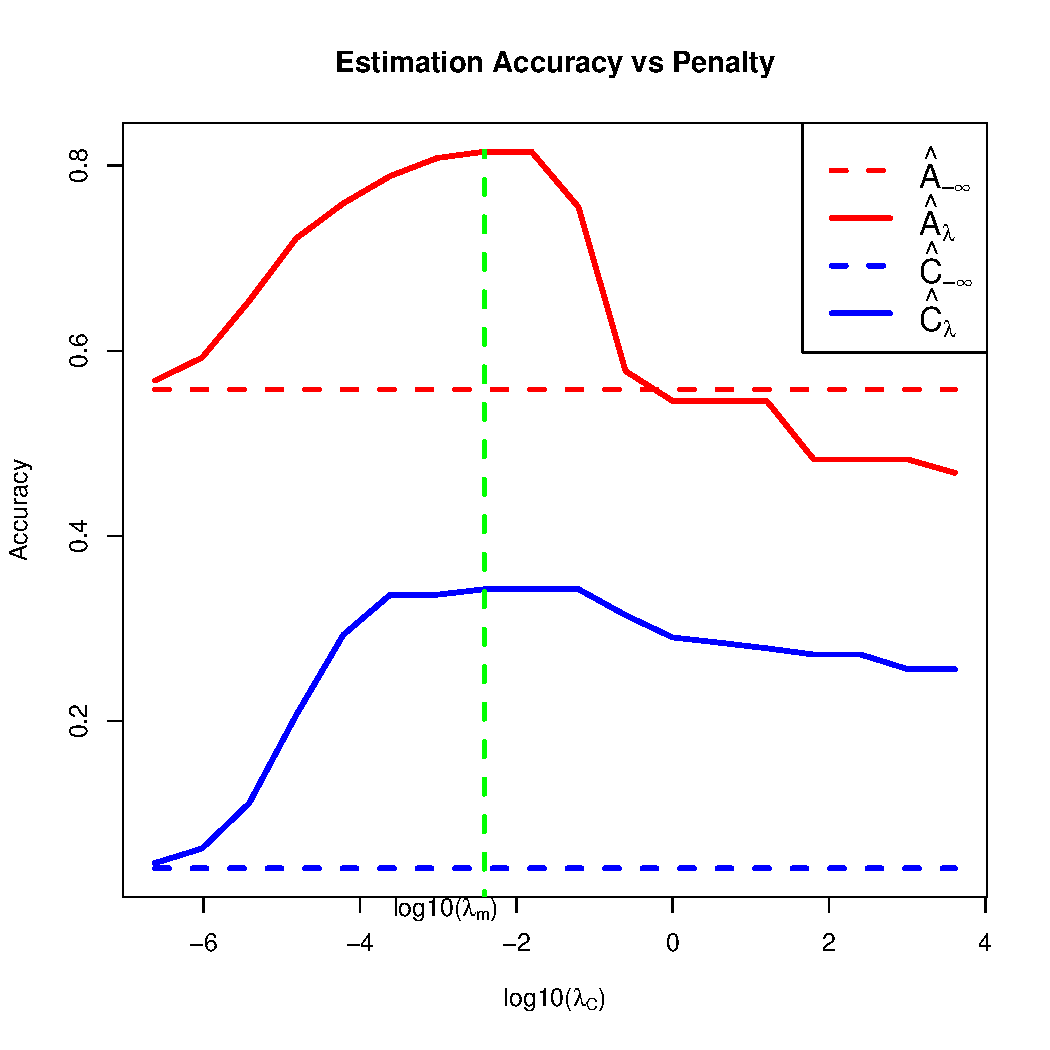
\includegraphics[scale=.43]{./figures/low-d-simulation.pdf}
}
\subfigure[High dimensional setting]{%
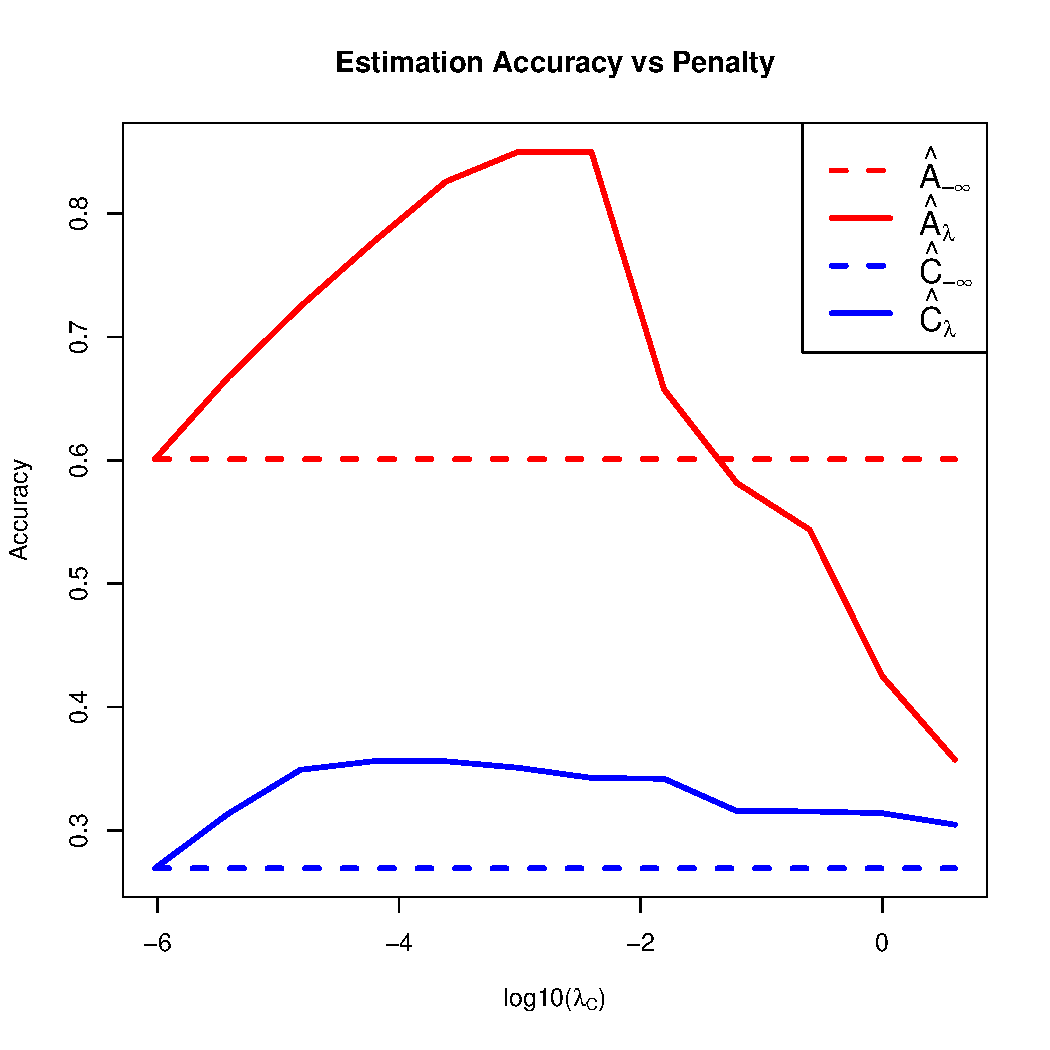
\includegraphics[scale=.43]{./figures/high-d-simulation.pdf}
}
\caption{x axis is tuning parameter $\lambda_C$ under log scale and y axis is the distance between truth and estimations; $\lambda_A$ is increasing proportionally with $\lambda_C$. One can see that in both the low dimensional and hight dimensional setting, estimation accuracies for $A$ and $C$ first increase then decrease as penalty increases..}
\label{fig:low-high-d-sim}
\end{figure}


As a concrete example, estimations from both methods are compared to the true values of parameters in Figure \oldref{fig:heatmap}. One can see that true values in each column of $C$ matrix are decreasing smoothly. $\hat{C}_{\lambda_m}$, which is estimated with optimal penalties $\lambda_C = \lambda_m$ and $\lambda_A = k\lambda_m$, shows similar pattern. In terms of $A$, the true value is sparse with many $0$ (blue) values. PLDS estimation $\hat{A}_{\lambda_m}$ is also sparse, denoted by the off-diagonal blue values. However, LDS estimation $\hat{A}_{\lambda_{-\infty}}$ is not sparse, with many yellow and red off-diagonal values.
\begin{center}
 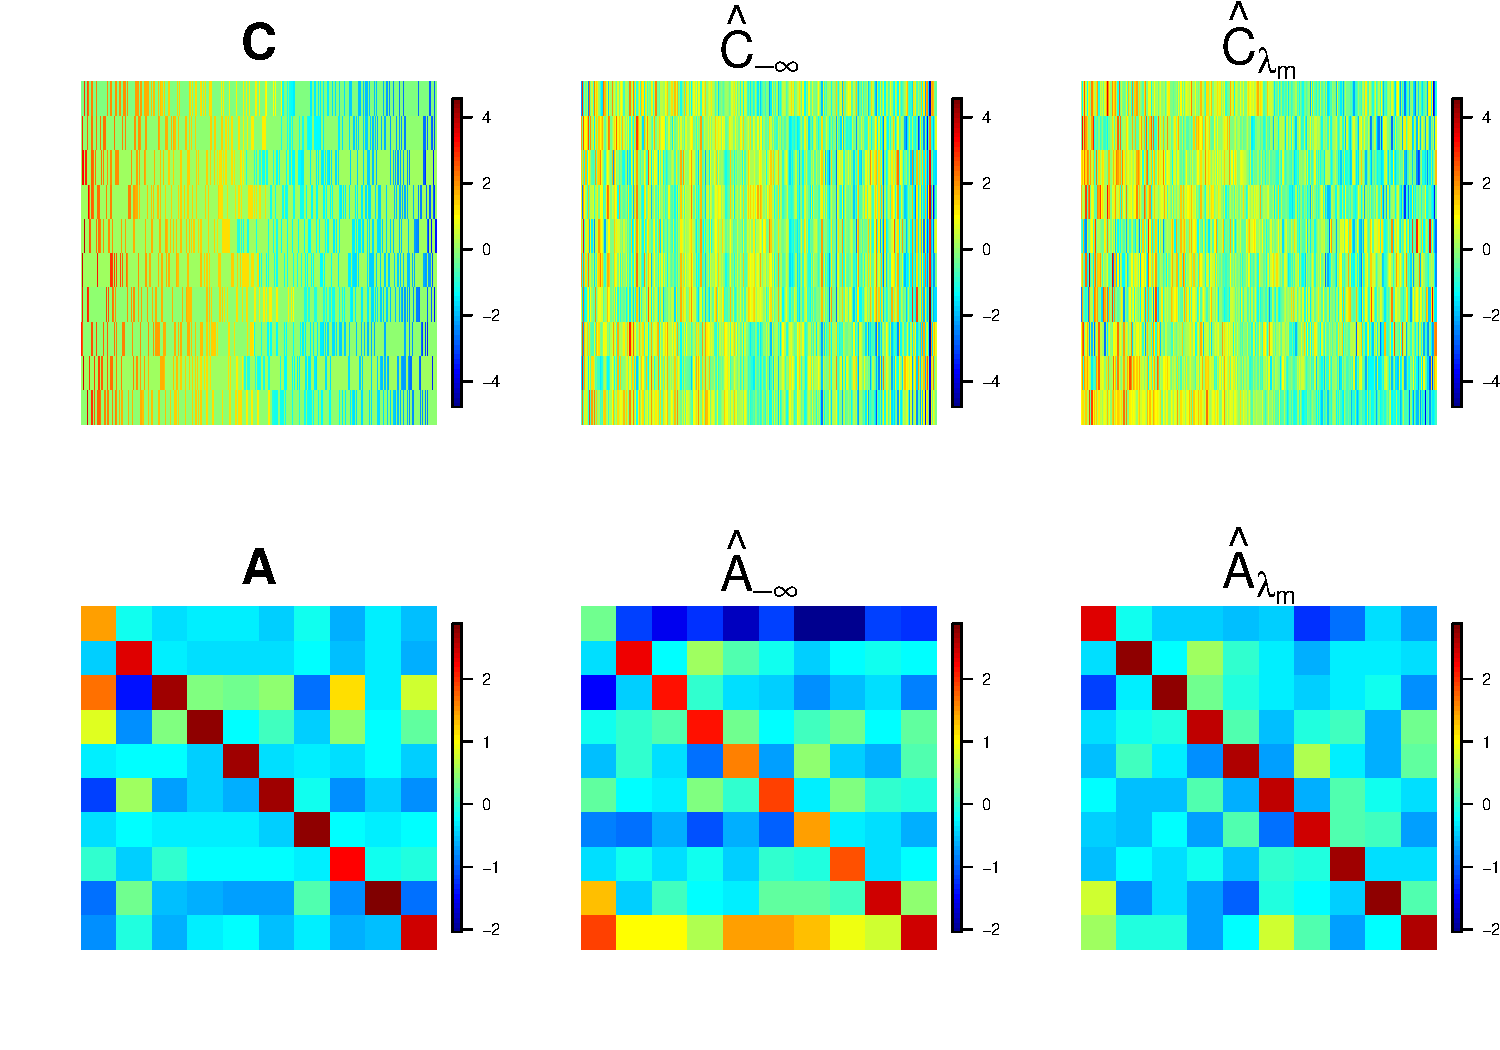
\includegraphics[scale=.6]{./figures/heatmap-figure-1}
 \captionof{figure}{Row 1: A truth; non-penalized estimation of A; optimally penalized estimation of A. Row 2: C truth; non-penalized estimation of C; optimally penalized estimation of C.}
 \label{fig:heatmap}
\end{center}



%The results are given in Figure \ref{fig:high-d-sim}; note the similar properties as in the low dimensional setting.
%\begin{center}
% 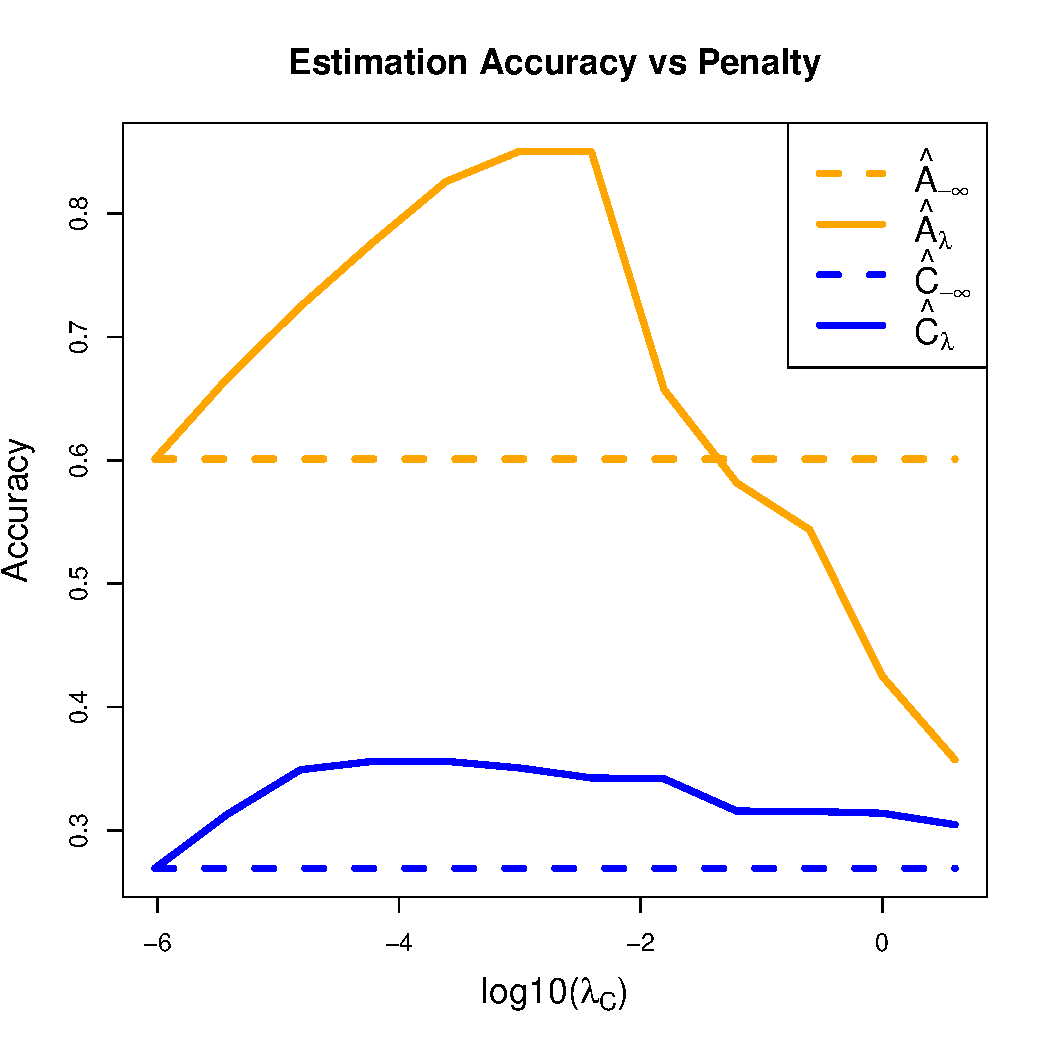
\includegraphics[scale=.6]{high-d-simulation.pdf}
%\captionof{figure}{Simulation Results: p = 10,000, d = 10 and T = 120; x axis is the penalty parameter under log scale with base 4 and y axis is the canonical correlation with true values of the parameters}
%\label{fig:high-d-sim}
%\end{center}

In addition to the improved estimation accuracy, the proposed algorithm is also computational efficiency and highly scalable. As a demonstration, we measure the running times of multiple simulation scenarios and summarize them in Table \oldref{tab:runningTime}. When both $p$ and $d$ are high dimensional, the algorithm can still solve the problem in a reasonable time.
\begin{center}
\captionof{table}{PLDS Running Time}
\label{tab:runningTime}
\begin{tabular}{c|ccccc}
\hline\hline
$p$ & 100 & 1000 & 10000 & 100000 & 100000\\
\hline
$d$ & 10 & 30 & 50 & 100 & 500 \\
\hline
$T$ & 100 & 300 & 500 & 1000 & 1000 \\
\hline
Time (min)& 0.04 & 0.50  & 51.28 & 208.82 & 1801.00 \\
\hline\hline
\end{tabular}
\end{center}
\subsection{Making Predictions}
Another perspective when considering PLDS model is its ability to make predictions. When the parameters $\mathbf{\Theta}$ and the latent states $x_T$ are estimated, one can first use estimated $x_T$ to predict $x_{T+1}$ and use $x_{T+1}$ to predict $y_{T+1}$. Similarly, more predictions $y_{T+2},\ldots, y_{T+k}$ can be made. Intuitively, properly chosen penalties give better estimations and good estimations should give more accurate predictions. This idea is demonstrated with a simulation. The parameter settings for this simulation follow Section \oldref{sec:lowdsim}. The correlation between the predicted signal and true signal is used as a measure of prediction accuracy. The prediction accuracy over penalty size is shown in Figure \oldref{fig:estpredaccuracy}.

%Specifically, the following simulation is performed: the proposed PLDS model is used to make 1-step, 2-step, $\cdots$, k-step predictions. Similar predictions are made with a PCA-based procedure and the prediction accuracies are compared.

%In the PCA-based procedure, denote $\mathbf{Y} = \left[\mathbf{y_1},\cdots,\mathbf{y_T}\right]$, a $p\times T$ matrix. The singular value decomposition (SVD) of $\mathbf{Y}$ is
%\begin{equation*}
%    \mathbf{Y} = \mathbf{UDV^{\prime}} = \mathbf{U}_{p\times T}\mathbf{X}_{T \times T}
%\end{equation*}
%Based on this decomposition, $\mathbf{U}_{p\times T}$ is used as the estimation of $C$ matrix, and the columns of $\mathbf{X}_{T \times T}$ are used in a vector autoregressive (VAR) model to estimate the coefficient matrix $A$. With an estimation for $C$ and for $A$, one can begin by computing a 1-step prediction for $\mathbf{x}_{T+1}$, then for $\mathbf{y}_{T+1}$. With these predictions, one could further generate the 2-step, 3-step, ..., k-step predictions.



\begin{center}
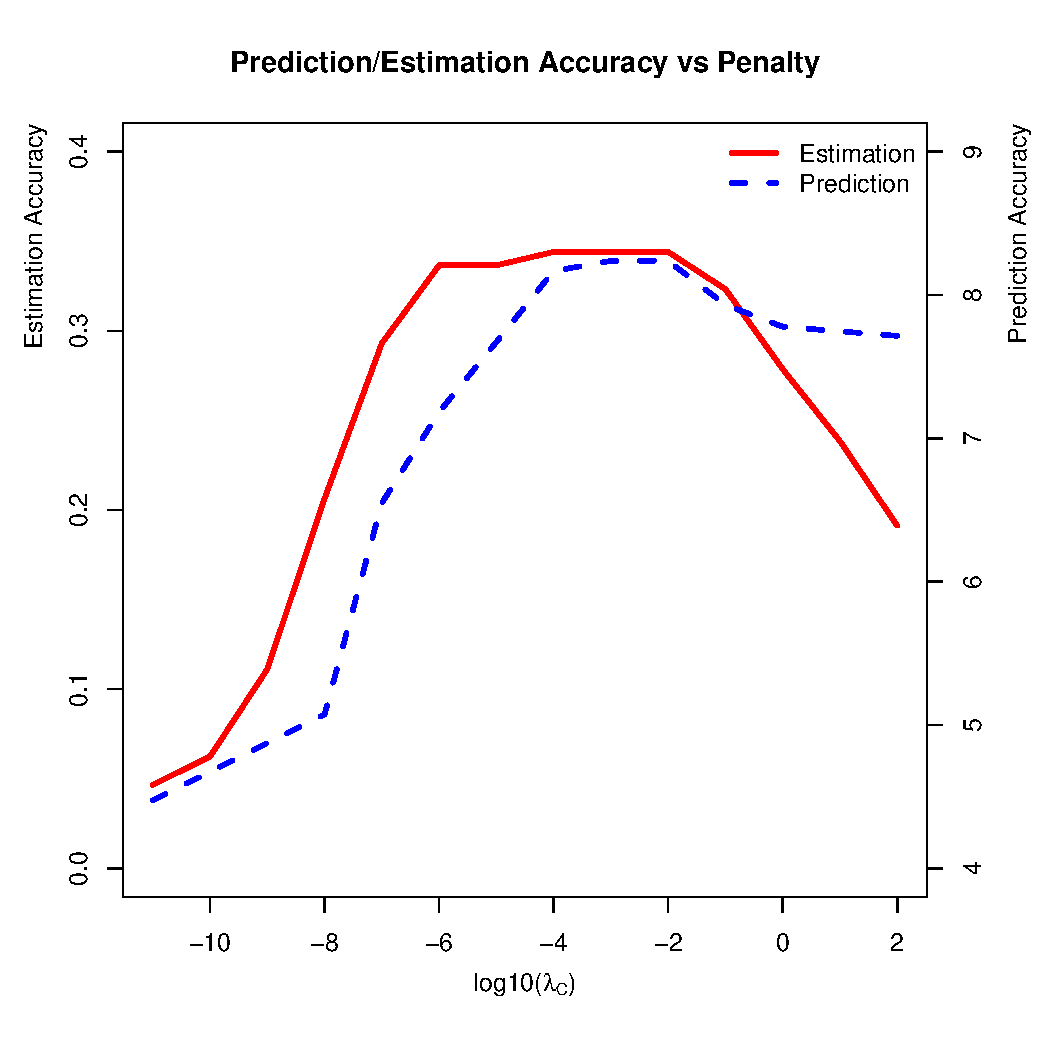
\includegraphics[scale=0.7]{./figures/est-pred-accuracy.pdf}
\captionof{figure}{Estimation and prediction accuracies.x axis is the penalty size under log scale, while y axis is the estimation and prediction accuracies. One can see that the penalty that yields the most accurate estimation also gives the best predictions.}
\label{fig:estpredaccuracy}
\end{center}

%\begin{center}
%\includegraphics[scale = 1.2]{prediction_accuracy-figure-3}
%\captionof{figure}{Left panel: prediction accuracy (the correlations between predictions and truth) versus penalty. Right panel: prediction accuracy versus estimation accuracy plot; the positive correlation is significant while the size of the circle represents penalty size.}
%\label{fig:predacrcy}
%\end{center}

Observations and findings from these plots include:
\begin{itemize}
 %\item PLDS prediction accuracy is almost the same as the PCA-based procedure when there is no penalty. This is consistent with the fact that the generic LDS is equivalent to PCA with some constraints on parameters.
 \item The prediction accuracy first improves then drops when the penalties increase
 \item The prediction accuracy peaks when the penalty coefficient $\lambda_A$ and $\lambda_C$ are around $10^{-3}$. This make sense as the same $\lambda$ pair also gives the best estimation for coefficients $A$ and $C$, as in Figure \oldref{fig:low-high-d-sim}.
\end{itemize}

This second observation provides us a way to pick tuning parameters in real applications, as detailed in Section \oldref{sec:application}.

%The concept that better estimations yields better predictions is further shown on the right panel of Figure \ref{fig:predacrcy}. One can see that the prediction accuracy and estimation accuracy are positively correlated and the correlation is significant. In addition, the size of top-right circles are neither over- or under-sized, which denotes that neither too large nor too small penalties yield best estimations or predictions. The main conclusion to draw from this simulation is that, better prediction can be achieved with properly chosen penalties.


\section{Application}
\label{sec:application}
When applied to fMRI data analysis, the model has very good interpretability. Each $\mathbf{y}_t$ is a scan of the brain. Each column of the $C$ matrix is interpreted as a time-invariant brain signal. At each time point, the observed brain image, $\mathbf{y}_t$, is a linear mixture of these networks and $\mathbf{x}_t$ explains how these networks are mixed at time $t$. Matrix $A$ describes how $\mathbf{x}_t$ evolves over time. $A$ can also be viewed as a directed graph if each network is treated as a vertex. Brain networks are spatially smooth and connectivities among them are empirically sparse. This naturally fits into the sparsity and smoothness assumptions in PLDS.

PLDS is applied to analyze the motor cortex of human brains from the KIRBY 21 Data. These data are resting-state fMRI scans consisting of a test-retest dataset previously acquired at the FM Kirby Research Center at the Kennedy Krieger Institute, Johns Hopkins University \cite{landman2011multi}. Twenty-one healthy volunteers with no history of neurological disease each underwent two separate resting state fMRI sessions on the same scanner: a 3T MR scanner utilizing a body coil with a 2D echoplanar (EPI) sequence and eight channel phased array SENSitivity Encoding (SENSE; factor of 2) with the following parameters: TR 2s; 3mm$\times$3mm in plane resolution; slice gap 1mm; and total imaging time of 7 minutes and 14 seconds.

In this application, test-retest scans from two subjects are analyzed. The imaging data are first preprocessed with FSL, a comprehensive library of analysis tools for fMRI, MRI and DTI brain imaging data \cite{smith2004advances}. FSL is used for spatial smoothing with Gaussian kernel. Then PLDS is applied on the smoothed data.

The following are basic descriptions of the data and model parameters.
\begin{itemize}[noitemsep, topsep=0pt]
\item Number of voxels, p = 7396
\item Number of scans, T = 210
\item Number of latent states, d = 11
\item Tuning parameters: $\lambda_A = 0.00001$, $\lambda_C = 0.00001$.\footnote{Different combinations of $\lambda_A$ and $\lambda_C$, where $\lambda_A = \lambda_C$ is applied to the data. The values range from $10^{-10}$ to $10^{4}$. Then the estimations are used to make predictions. The combination that gives the best predictions is used here. One can also use a grid of combinations, but it is time consuming.}
\item Max number of iterations: EM 30 steps, L-1/L-2 regularized subproblems, 30 steps
\end{itemize}

The number of latent states, d, can be manually selected based on related research that maps the primary motor region to human activities. For instance, Meier et al. mapped the motor region to 9 human organs: tongue, lips, squint, fingers, wrist, forearm, elbow, foot and saccade \cite{meier2008complex}.

A more flexible technique to choose the number of latent states involves the profile likelihood method proposed by Zhu et al. \cite{zhu2006automatic}. As a first step, eigenvalues of the data matrix are calculated with Principal Component Analysis (PCA). The cumulative eigenvalues as a percentage of the sum of all eigenvalues are then plotted - see Figure \oldref{fig:eigvals}. Visually one notes that the first 10 eigenvalues take over $80\%$ of all variations. The number of latent states can be selected as the smallest number (of eigenvalues) that explains over $80\%$ of total variation in the data. However, the drawback of this method is clear: the choice of threshold percentage (here $80\%$) is highly subjective. The profile likelihood method overcomes this problem and could pick the dimension automatically.

The above method assumes that the first $k$ eigenvalues are samples from a Gaussian distribution $N(\mu_1,\sigma^2)$, while the rest are from a different Gaussian distribution $N(\mu_2,\sigma^2)$. Then the profile likelihood can be calculated given $k$, for all $k=1,\cdots,T$ and selecting the optimal $k$ as the one with the highest profile likelihood. As shown in Figure \oldref{fig:eigvals}, when the profile likelihood method is applied to the first scan of subject one, d = 11 is selected. Apply the method to all four scans, the numbers of latents states selected are 11, 6, 14 and 15 respectively. Their average, $d=11$, is used.

\begin{center}
\[
\begin{array}{cc}
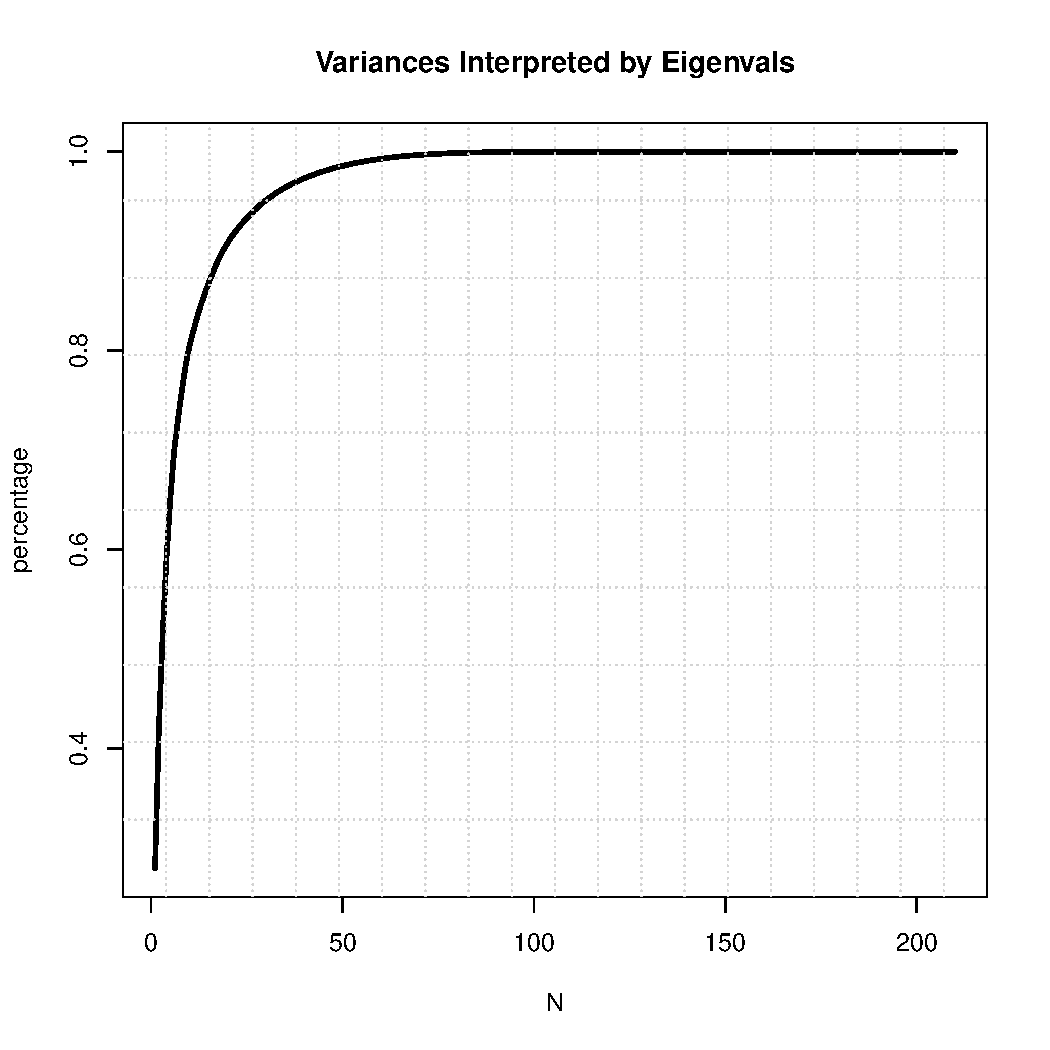
\includegraphics[scale = 0.45]{./figures/EigenValues.pdf} & 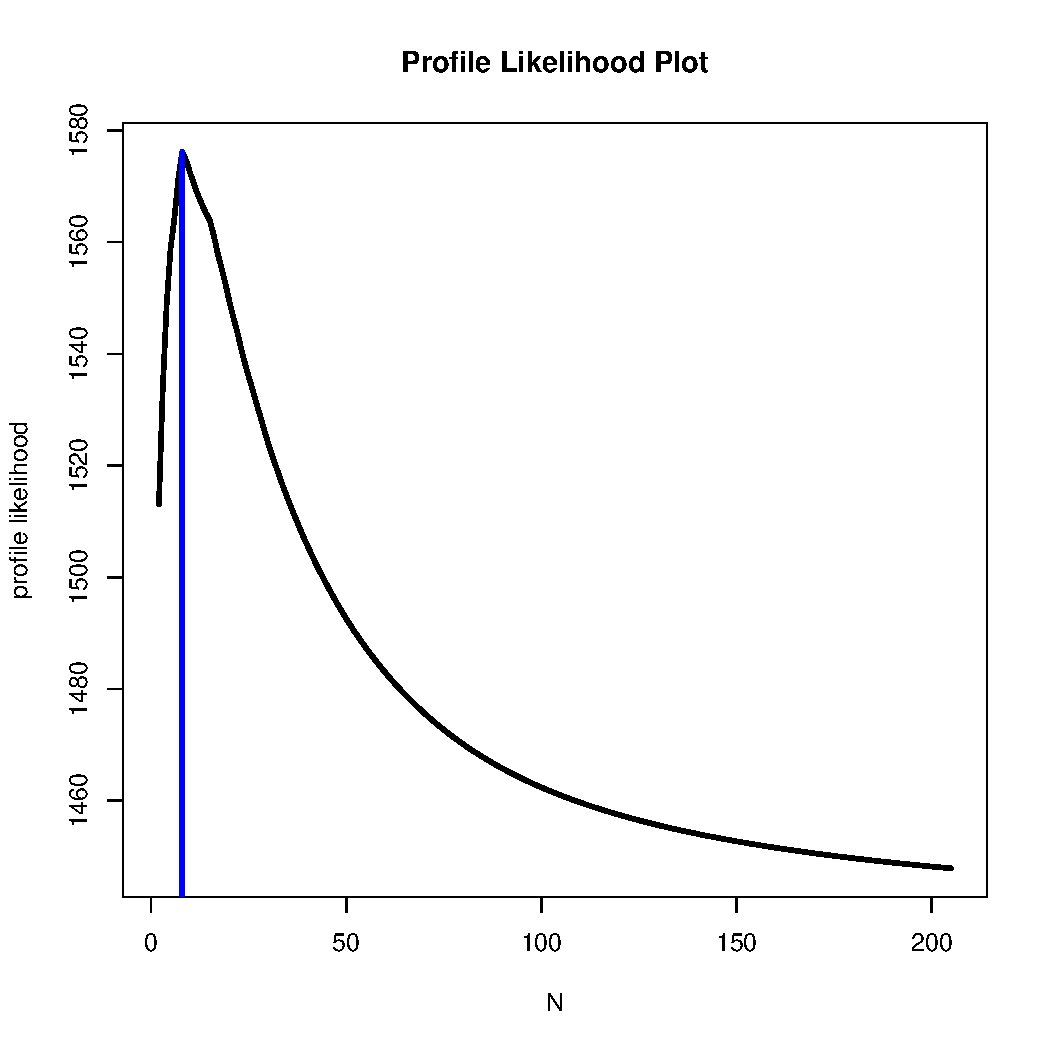
\includegraphics[scale=0.45]{./figures/profileLikelihood.pdf}
\end{array}
\]
\captionof{figure}{Eigen-values and corresponding profile likelihood plot from the first scan of subject one. For this data, the profile likelihood picks $d=11$ as the number of latent states.}
\label{fig:eigvals}
\end{center}


% One can group the scans correctly with the $A$ matrices.
Denote the $A$ matrix estimation for the second scan of subject one as $A_{12}$. Similar notations apply to the other scans. Then the canonical correlations among the four matrices are summarized in Table \oldref{tab:similarity}. The distance measure in Equation \ref{eq:distance} is used. Another permutation invariant measure of distance between two square matrices, the Amari error \cite{amari1996new}, is also provided in the table \footnote{The Amari error between $A$ and $\hat{A}$: $E(A,\hat{A}) = \sum\limits_{i=1}^n(\sum\limits_{j=1}^n\frac{|p_{ij}|}{\max_k |p_{ik}|}-1) + \sum\limits_{j=1}^n(\sum\limits_{i=1}^n\frac{|p_{ij}|}{\max_k|p_{kj}|}-1)$, where $P =(p_{ij})=A^{-1}\hat{A}$.}. Notice a smaller $d(A,B)$ or Amari error means more similarity. Among the six pairs from $A_{11},A_{12},A_{21}$ and $A_{22}$, it is expected that the pairs $(A_{11},A_{12})$ and $(A_{21},A_{22})$ give the smallest distances, as each pair comes from two scans of the same subject. This idea is validated by Table \oldref{tab:similarity}. A direct application of this result is to correctly cluster the four scans into two group, each group corresponding to a subject. This implies that the A matrices contains subject-specific information. The $A$ matrices as connectivity graphs are plotted in Figure \oldref{fig:cgraph}.
\begin{center}
%\includegraphics[scale = 0.7]{ConnectivityGraph.pdf}
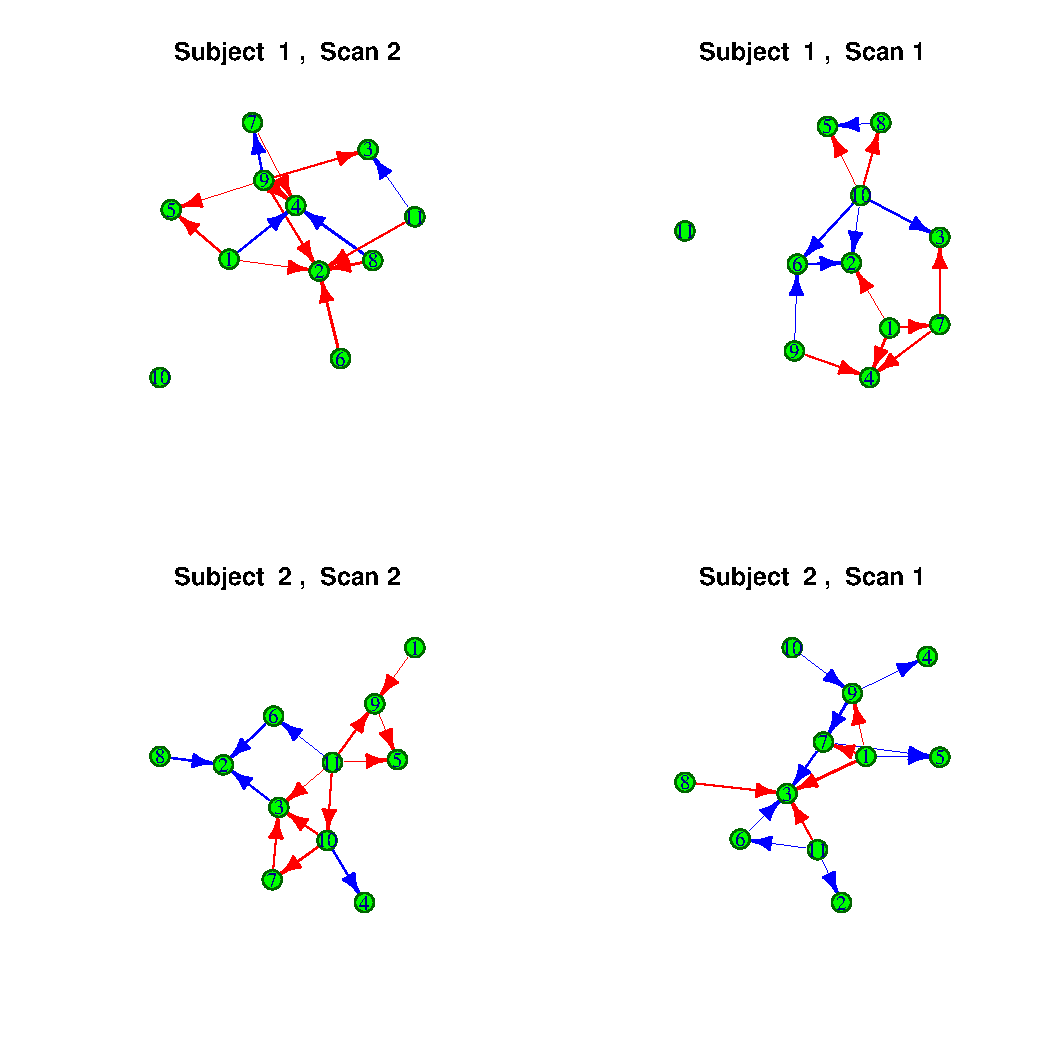
\includegraphics[scale = 0.85]{./figures/ConnectivityGraph_11_all.pdf}
\captionof{figure}{Connectivity Graph: The wider edge means stronger connectivity; the red edge means negative connectivity and blue edge means positive connectivity.}
\label{fig:cgraph}
\end{center}

%\begin{table}
%\centering
%\captionof{table}{Similarities Among Estimated $A$ Matrices}
%\label{tab:similarity}
%\begin{tabular}{c|c|c|c|c|c|c}
%\hline\hline
%Pairs & $A_{11},A_{12}$ & $A_{11},A_{21}$ & $A_{11},A_{22}$ & $A_{12},A_{21}$ & $A_{12},A_{22}$ & $A_{21},A_{22}$\\
%\hline
%$d(\cdot,\cdot)$ & $\mathbf{10.2}$ & $9.9$ & $10.0$ & $10.0$ & $10.0$ & $\mathbf{10.1}$ \\
%Amari Error & $\mathbf{0.88}$ & $1.05$ & $1.02$ & $1.08$ & $1.09$ & $\mathbf{0.98}$ \\
%\hline
%\end{tabular}
%\end{table}

\begin{table}
\centering
\captionof{table}{Similarities Among Estimated $A$ Matrices}
\label{tab:similarity}
\begin{tabular}{c|cccc}
\hline
$d(\cdot,\cdot)$(Amari Error) & $A_{11}$&$A_{12}$ & $A_{21}$&$A_{22}$ \\
\hline
$A_{11}$ & $0$ &  &  &\\
$A_{12}$ & $\mathbf{0.076(0.88)}$& $0$ & &\\
$A_{21}$ & $0.105(1.05)$ & $0.095(1.08)$  & $0$ &\\
$A_{22}$ & $0.095(1.02)$ & $0.095(1.09)$ & $\mathbf{0.085(0.98)}$ & $0$ \\
\hline
\end{tabular}
\end{table}

The similarities among $A$ matrices are also shown in Figure \ref{fig:matsim} as a heatmap.
\begin{center}
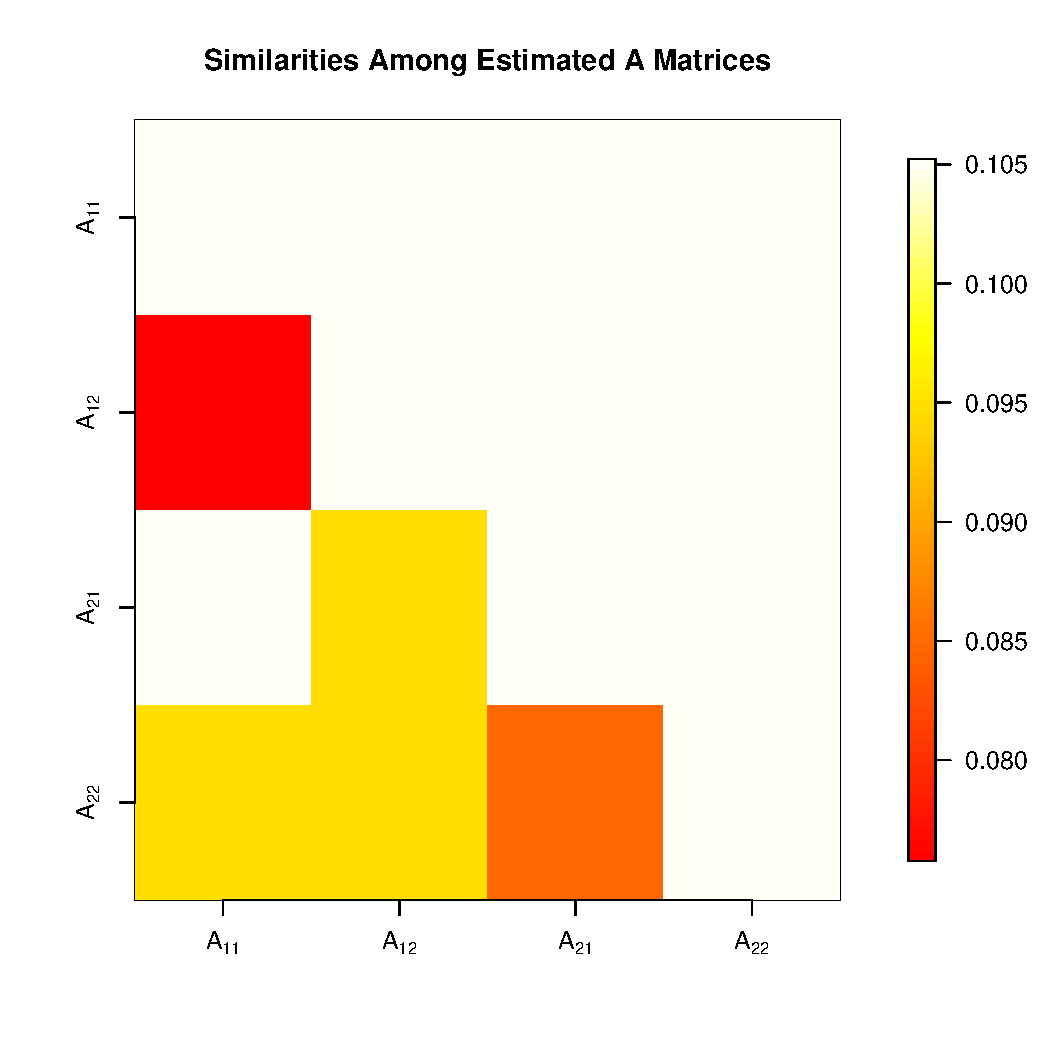
\includegraphics[scale=.5]{./figures/A-matrices-similarity.pdf}
\captionof{figure}{Similarities among the four estimated $A$ matrices. The distance $d(\cdot,\cdot)$ is used in this figure. As one can see, the two red/orange off-diagonal pixels has the minimum distances, which correspond to the pairs of $(A_{11},A_{12})$ and $(A_{21},A_{22})$ respectively. With this similarity map, one can tell which two scans are from the same subject.}
\label{fig:matsim}
\end{center}

As an example, the 3D renderings of the columns of matrix $C$ from the first scan of subject one are shown in Figure \oldref{fig:3d} (after thresholding). The biological meaning of those regions need to be further validated. It is helpful to compare those regions to other existing parcellations of the mortor cortex. As an example, the blue region in Figure \oldref{fig:3d} accurately matches the dorselmedical (DM) parcel of the five-region parcellation proposed by Nebel MB et al. \cite{nebel2014disruption}.
\begin{center}
\[
\begin{array}{lll}
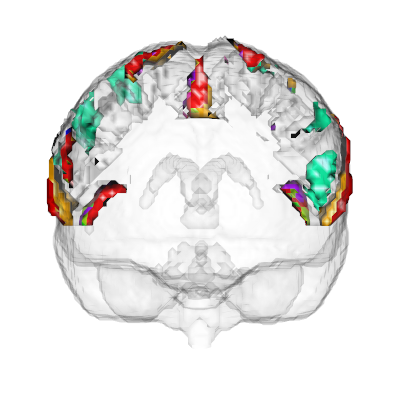
\includegraphics[scale = 0.36]{./figures/view1.png} & 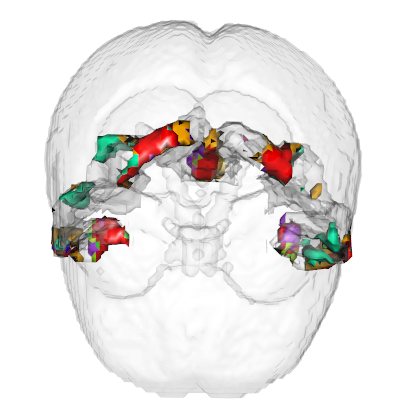
\includegraphics[scale = 0.33]{./figures/view2.png} & 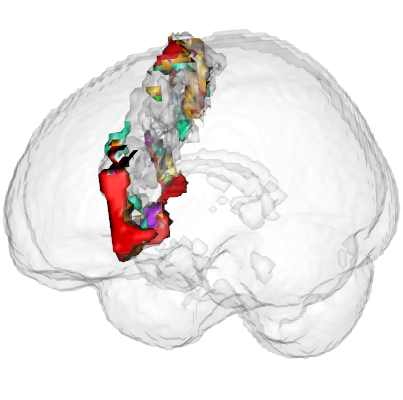
\includegraphics[scale = 0.33]{./figures/view3.png}
%\includegraphics[scale = 0.21]{view1-26.png} & \includegraphics[scale = 0.21]{view2-26.png} & \includegraphics[scale = 0.21]{view3-26.png}
\end{array}
\]
\captionof{figure}{3D rendering of columns of matrix $C$: estimation from the first scan of subject one shown in this plot.}
\label{fig:3d}
\end{center}

Another application of the algorithm is predicting brain signals. To demonstrate this, the algorithm is applied to the Human Connectome Project (HCP) data. (\textbf{Descriptions of data and citations required here})

Using the profile likelihood method, $d=149$ is picked. The data has $T=1200$ time points. The first $N = 1000$ are picked as training data, while the rest are used as test data. Then both the SVD method in Section \oldref{sec:initial} and PLDS algorithm are used for estimations. Then $k$-step ahead predictions are made with equations \ref{eq:model0} and estimations from both methods. Pseudocode for $k$-step ahead predictions is given in Appendix 3. The prediction accuracies are shown in Figure \oldref{fig:predaccy}. The first observation is that, PLDS algorithm is giving significantly better predictions for the first 150 predictions compared to the SVD method. As the SVD method is also used to intialize PLDS algorithm, this shows that PLDS algorithm improves estimations from the SVD method in terms of short-term predictions. Another observation is, PLDS algorithm's performance get worse when one predicts into the ``long" future ($>150$ steps). This is reasonable because the prediction errors from each step will accumulate and yields deteriorating predictions as the number of steps increase.

\begin{center}
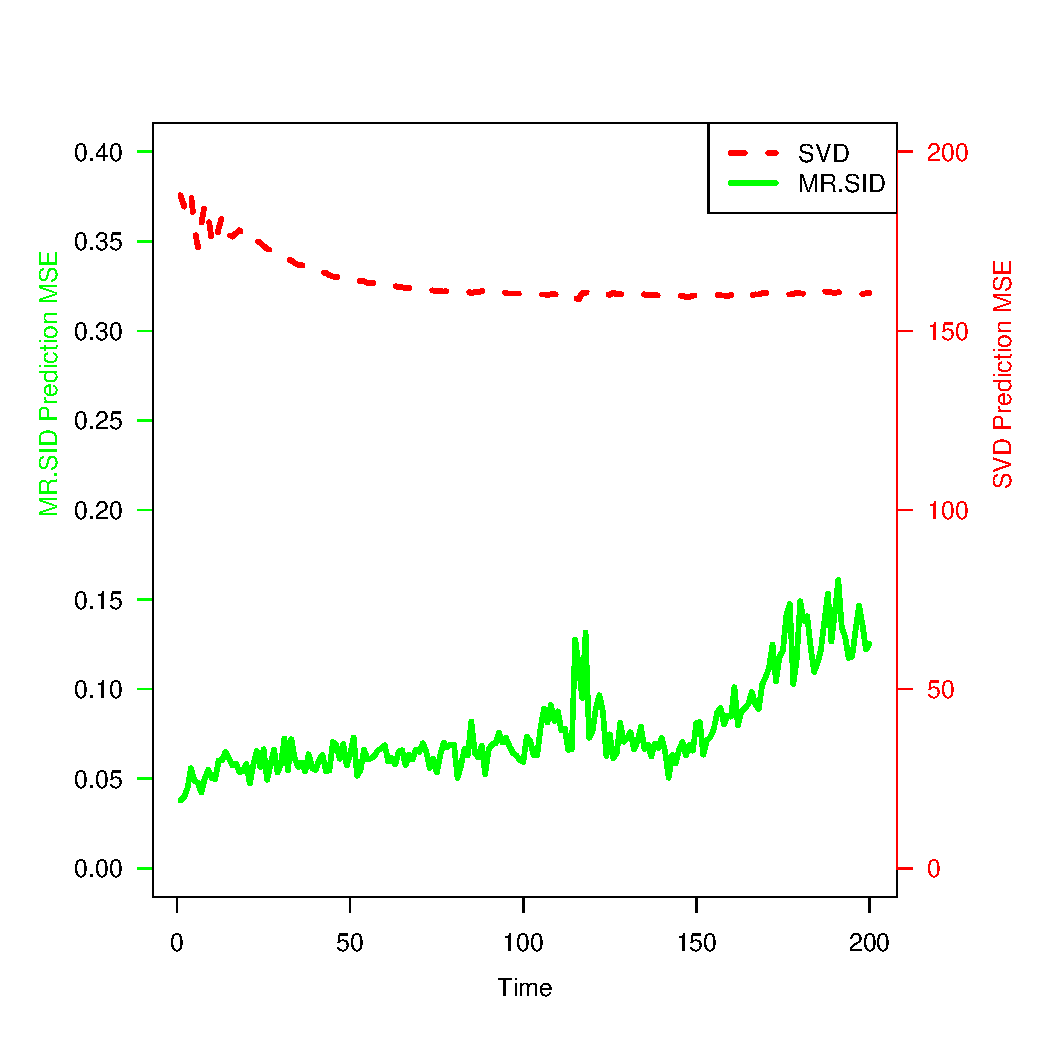
\includegraphics[scale=0.5]{./figures/hcp_pred_accy.pdf}
\captionof{figure}{Prediction accuracies comparison on HCP data. The mean squared error (MSE) is used as the accuracy measure.}
\label{fig:predaccy}
\end{center}

A sample plot of the true time series and predicted values are shown in Figure \oldref{fig:samplets}. We see that PLDS is giving more accurate predictions and the true signal lies in the confidence band giving by PLDS model. Another observation is that the confidence band is getting wider as we predict into the future, which is a result of the accumulated errors.

\begin{center}
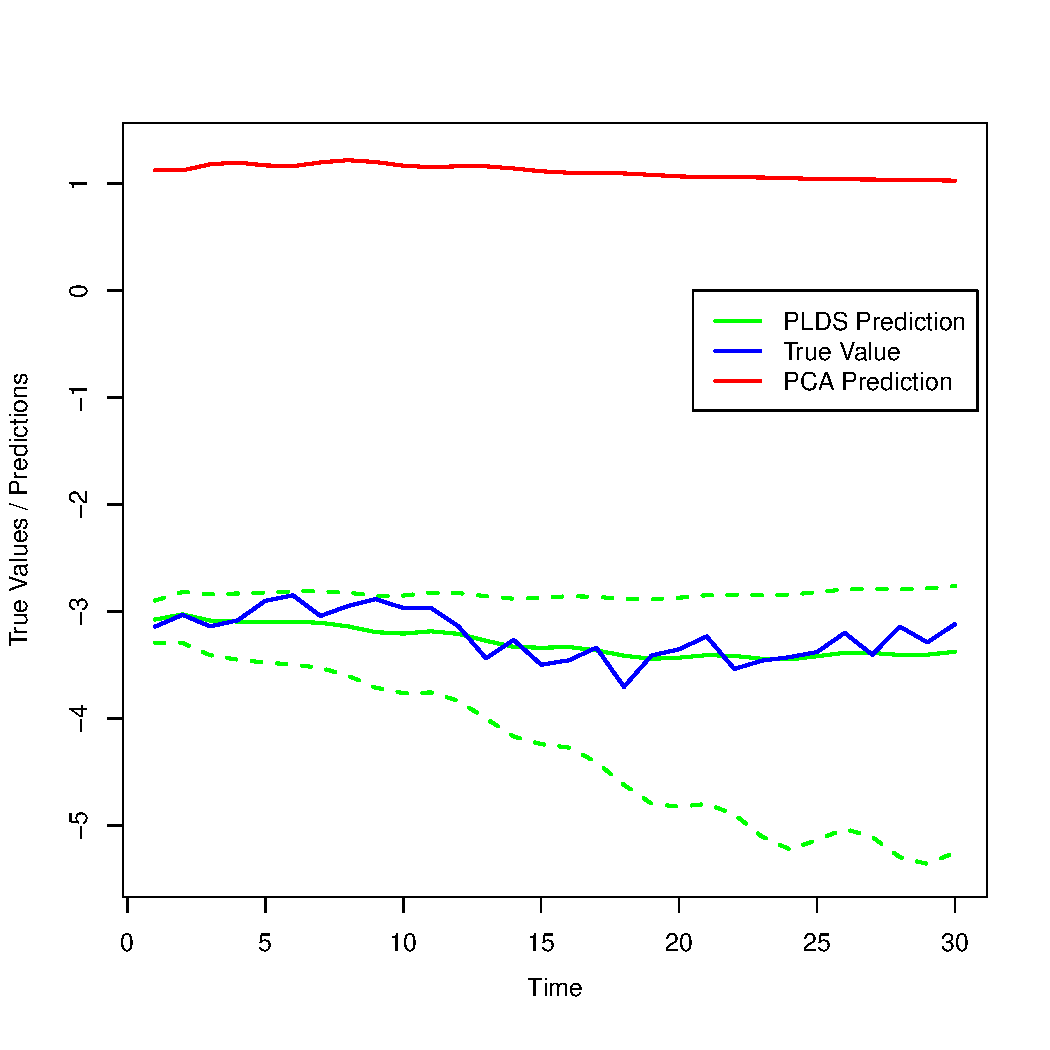
\includegraphics[scale=0.5]{./figures/newSampleTS.pdf}
\captionof{figure}{Sample time series plot. The dotted green curve stands for the $60\%$ confidence band given by PLDS model. The true time series is averaged signals from a subsample of voxels. The predictions are also averaged over the same subsample. The confidence band is estimated based on the covariance matrix of these voxels. A subsample of 20 voxels are picked in this experiment to avoid big covariance matrices calculation. All values are log-scaled for plotting purpose.}
\label{fig:samplets}
\end{center}

%The columns of matrix $C$ is explored as follows.
%\[
%\begin{array}{ccc}
%\includegraphics[scale=0.3]{1.png}&\includegraphics[scale=0.3]{2.png}&\includegraphics[scale=0.3]{3.png}\\
%\includegraphics[scale=0.3]{4.png}&\includegraphics[scale=0.3]{5.png}&\includegraphics[scale=0.3]{6.png}\\
%\includegraphics[scale=0.3]{7.png}&\includegraphics[scale=0.3]{8.png}&\includegraphics[scale=0.3]{9.png}\\
%\end{array}
%\]

%\begin{center}
%\captionof{figure}{Thresholded Connectivity Graphs(Left: Nonpenalized; Right: Penalized)}
%\includepdf[scale=0.8]{kfs-connectivity.png}
%\end{center}
%
%\begin{center}
%\captionof{figure}{Thresholded Connectivity Graphs(Left: Nonpenalized; Right: Penalized)}
%\includepdf[scale=0.8]{pkfs-connectivity.png}
%\end{center}
%\subsection{eigenvalues Of Data Matrix}
%The eigenvalues plot is given in the following figure
%\begin{center}
%\includegraphics[scale=0.7]{eigvals.png}
%\end{center}
%The two solid lines represents subject 1 and the other two dashed lines represent subject 2. Each subject has two scan sessions.
\section{Discussion}
By applying the proposed model to fMRI scans of the motor cortex of healthy adults, we identify limited sub-regions (networks) from the motor cortex. A statistical procedure should be further developed to match these regions to existing parcellations of the motor cortex.

In the future, this work could be extended in two important directions. First, assumptions on the covariance structures in the observation equation could be generalized. Prior knowledge could be incorporated to covariance $R$. The general rule is that $R$ should be general enough to be flexible while sufficiently restricted to make the model useful. A lot of other platforms such as tridiagnol and upper triangular could also be considered. Mohammad et al. have discussed the impact of auto correlation on functional connectivity, which also provides us a direction for extension \cite{arbabshirani2014impact}.

Finally, the work can also be extended on the application side. Currently, only data from a single subject is analyzed. As a next step, the model can be extended to a group version and be used to analyze more subjects. The coefficients from the algorithm could be used to measure the reproducibility of the scans.

\section*{Appendix 1}
\label{sec:appendix1}

\begin{tabular}{l}
\hline
\textbf{Algorithm } Standard Kalman Filter Smoother for estimating the moments \\
$\qquad\quad\quad$ required in the E-step of an EM algorithm for a linear dynamical system\\
\hline
0. Define $\mathbf{x}_t^{\tau}$ = E($\mathbf{x}_t|\{\mathbf{y}\}_1^{\tau}$),$\mathbf{V}_t^{\tau}=\text{Var}(\mathbf{x}_t|\{\mathbf{y}\}_1^{\tau})$, $\hat{\mathbf{x}}_t \equiv \mathbf{x}_t^T$ and $P_t\equiv V_t^T+\mathbf{x}_t^T{\mathbf{x}_t^T}^{\T}$\\
1. Forward Recursions:\\
\hspace{4 mm} $\mathbf{x}_t^{t-1}=A\mathbf{x}_{t-1}^{t-1}$\\
\hspace{4 mm} $\mathbf{V}_t^{t-1}=A\mathbf{V}_{t-1}^{t-1}+\mathbf{Q}$\\
\hspace{4 mm} $K_t=\mathbf{V}_t^{t-1}C^{\T}(CV_t^{t-1}C^{\T}+R)^{-1}$\\
\hspace{4 mm} $\mathbf{x}_t^t$ = $\mathbf{x}_t^{t-1} + K_t (\mathbf{y}_t - C\mathbf{x}_t^{t-1})$\\
\hspace{4 mm} $V_t^t=V_t^{t-1}-K_tCV_t^{t-1}$\\
\hspace{4 mm} $\mathbf{x}_1^0=\mathbf{\pi}_0$, $V_1^0=\mathbf{V}_0$\\
2. Backward Recursions:\\
\hspace{4 mm} $J_{t-1} = V_{t-1}^{t-1}A^{\T}(V_t^{t-1})^{-1}$\\
\hspace{4 mm} $\mathbf{x}_{t-1}^T=\mathbf{x}_{t-1}^{t-1}+J_{t-1}(\mathbf{x_t^T-A\mathbf{x}_{t-1}^{t-1}})$\\
\hspace{4 mm} $V_{t-1}^T = V_{t-1}^{t-1}+J_{t-1}(V_t^T-V_t^{t-1})J_{t-1}^{\T}$\\
\hspace{4 mm} $P_{t,t-1}\equiv V_{t,t-1}^T+\mathbf{x}_t^T{\mathbf{x}_t^T}^{\T}$\\
\hspace{4 mm} $V_{T,T-1}^T=(I-K_TC)AV_{T-1}^{T-1}$\\
\hline
\end{tabular}

\newpage

\section*{Appendix 2}
\label{sec:appendix2}
In general, FISTA optimize a target function
\begin{equation}\label{eqn: fistatarget}
\min_{\substack{x\in \mathcal{X}}}\quad \mathbf{F(x;\lambda)} = \mathbf{g(x)}+ \mathbf{\lambda \|x\|_1}
\end{equation}
where $\mathbf{g}: R^n \rightarrow R $ is a continuously differentiable convex function and $\lambda > 0$ is the regularization parameter.
%\begin{itemize}
%\item $\mathbf{f}: R^n \rightarrow R $ is continuously differentiable convex function
%\item $\lambda > 0$ is the regularization parameter
%\end{itemize}

A FISTA algorithm with constant step is detailed below\\

%\begin{center}
\begin{tabular}{l}
\hline
\textbf{Algorithm } FISTA$(\mathbf{g},\lambda)$.\\
\hline
 1. Input an initial guess $\mathbf{x_0}$ and Lipschitz constant $\mathbf{L}$ for $\mathbf{\nabla g}$, set $\mathbf{y_1} = \mathbf{x_0},t_1 = 1$\\
 2. Choose $\tau \in (0,1/\mathbf{L}]$.\\
 3. Set $k \leftarrow$ 0.\\
 4. \textbf{loop}\\
 5. \hspace{10mm}		Evaluate $\mathbf{\nabla g(y_k)}$\\
 6.	\hspace{10mm}	Compute $\mathbf{x_{1}}$= $\mathbf{S_{\tau\lambda}(y_k - \tau\nabla g(y_k))}$\\
 7.	\hspace{10mm}	Compute $t_{k+1} = \frac{1+\sqrt{1 + 4 t_k^2}}{2}$\\
 8.	\hspace{10mm}	$\mathbf{y_{k+1}} = \mathbf{x_k} + \left(\frac{t_k - 1}{t_{k+1}})\right (\mathbf{x_k}-\mathbf{x_{k-1}})$\\
 9.	\hspace{10mm}	Set $k \leftarrow k+1$ \\
 10. \textbf{end loop}\\
\hline
\end{tabular}
%\end{center}


\vspace*{10mm}
In the above
\[
\mathbf{S_\lambda (y) = (|y|-\lambda)_{+}\textbf{sign}(y)}=\left\{
\begin{array}{l l }
 y - \lambda & \text{if   } y > \lambda\\
 y + \lambda & \text{if   } y < -\lambda\\
 0 & \text{if   } |y| \leq \lambda .
\end{array}
\right.
\]

\section*{Appendix 3}

\begin{tabular}{l}
\hline
\textbf{Algorithm } $k$-step predictions with PCA and PLDS\\
\hline
 1. Denote the estimated parameters with PCA and PLDS as $A_{pca},C_{pca},A_{plds},$ and $C_{plds}$ respectively.\\
 2. PCA Estimated latent states at $t=1000$: $x_{1000,pca} = $ the $1000$th column of $\mathbf{X}_{d\times T}$ from Section \oldref{sec:initial} \\
 3. PLDS Estimated latent states at $t=1000$: $x_{1000,pls}$ is from E step of the EM algorithm in Section \oldref{sec:em}\\
 4. \textbf{for i = 1 to k}\\
 5. \hspace{10mm}		$x_{1000+k,pca}\ =\ A_{pca}\ x_{999+k,pca}$\\
 6.	\hspace{10mm}	$y_{1000+k,pca}\ =\ C_{pca}\ x_{1000+k,pca}$\\
 7.	\hspace{10mm}	$x_{1000+k,plds}\ =\ A_{plds}\ x_{999+k,plds}$\\
 8.	\hspace{10mm}	$y_{1000+k,plds}\ =\ C_{plds}\ x_{1000+k,plds}$\\
 9. \textbf{end}\\
\hline
\end{tabular}
\newpage
\bibliographystyle{plain}
\bibliography{reference}
\end{document}
